%!TEX TS-program = xelatex

%\pdfoutput=1

% IRI report class
%\documentclass{iritr}
%\IRIreport{18}{01}
%\coriri{Joan Sol\`a}{1 7337}{jsola}


%%%%%%%%%%%%%%%%%%%%%%%%%%% doc class %%%%%%%%%%%%%%%%%%%%%%%%%%%
% IEEE
\documentclass{IEEEtran}
\usepackage[fontset=founder]{ctex} % 增加中文格式的支持。
%\usepackage[fontset=founder,11pt]{ctex} % 小字体,紧凑一点。
\linespread{1.2}

% Article
%\documentclass[11pt]{article}
%\usepackage{a4wide}
%\usepackage{appendix}

%%%%%%%%%%%%%%%%%%%%%%%%%%% packages %%%%%%%%%%%%%%%%%%%%%%%%%%%%

\usepackage[english]{babel}
\usepackage{amsfonts, amssymb, amsmath} 
\usepackage{bm} 
%\usepackage{cancel}
\usepackage{mathtools}
%\usepackage{multirow}
\usepackage[ruled,vlined]{algorithm2e}

\usepackage{lastpage} % Count nbr of pages
\usepackage{balance}  % equalize columns in last page

\usepackage{xparse}

% For example boxes
\usepackage{mdframed}
\mdfsetup{skipabove=0pt,skipbelow=-2pt}
\usepackage{float}

% For prettier tables
\usepackage{booktabs} 

% Latex drawing
\usepackage{tikz}
\usetikzlibrary{positioning}


% Customization packages
\usepackage{customCommands} % Joan Sola's macros


% Define new plus and minus operators with diamond shape
\usepackage{scalerel}
\def\dplus{\,\scalerel*{
\includegraphics{./symbols/dplus.pdf}}{X\rule[-.5ex]{0pt}{1pt}\rule[1.4ex]{0pt}{1pt}}\,}
\def\dminus{\,\scalerel*{
\includegraphics{./symbols/dminus.pdf}}{X\rule[-.5ex]{0pt}{1pt}\rule[1.4ex]{0pt}{1pt}}\,}

\renewcommand\Re{\operatorname{Re}}
\renewcommand\Im{\operatorname{Im}}

% Comments
\newcommand{\COM}[1]{{\color{red}#1}}
%\renewcommand{\COM}[1]{}

% Define a few useful shortcuts
\newcommand{\bw}{{\bfomega}}
\newcommand{\bth}{{\bftheta}}
\newcommand{\bphi}{{\bfphi}}
\newcommand{\nth}{\norm{\bth}}
\newcommand{\ab}{{\bfa_b}}
\newcommand{\wb}{{\bw_b}}
\newcommand{\D}{\Delta}
\newcommand{\Dzero}{{\D^0}}
\newcommand{\Dp}{{\D\bfp}}
\newcommand{\Dv}{{\D\bfv}}
\newcommand{\Dth}{{\D\bth}}
\newcommand{\Dq}{{\D\bfq}}
\newcommand{\DR}{{\D\bfR}}
\newcommand{\DP}{{\D\bfP}}
\newcommand{\DV}{{\D\bfV}}
\newcommand{\DTH}{{\D\bfTheta}}
\newcommand{\Dw}{{\D\bw}}
\newcommand{\DW}{{\D\bfOmega}}
\newcommand{\dpp}{{\delta\bfp}}
\newcommand{\dv}{{\delta\bfv}}
\newcommand{\dth}{{\delta\bth}}
\newcommand{\dq}{{\delta\bfq}}
\newcommand{\dR}{{\delta\bfR}}
\newcommand{\dP}{{\delta\bfP}}
\newcommand{\dV}{{\delta\bfV}}
\newcommand{\dTH}{{\delta\bfTheta}}
\newcommand{\dw}{{\delta\bw}}
\newcommand{\hhat}{^\wedge}
\newcommand{\vvee}{^\vee}

\newcommand{\mtan}[1]{T#1}
\newcommand{\mtanat}[2]{T_{#2}{#1}}

% Derivatives and Jacobians
% -----------------------------------------
\renewcommand{\mjac}[2]{\jac{#1}{#2}} % Do not use fancy style for jacs in manifold

\newcommand{\der}{D}
%\newcommand{\der}{\partial}
\newcommand{\ndpar}[2]{\frac{\der#1}{\der#2}}
\NewDocumentCommand{\dparat}{ O{} O{} m m}{\frac{{^{#1}}\der#3}{{^{#2}}\der#4}}
\renewcommand{\rdpar}[2]{\dparat[#2][]{#1}{#2}}
\renewcommand{\ldpar}[2]{\dparat[\cE][]{#1}{#2}}
\newcommand{\rldpar}[2]{\dparat[#1][\cE]{#1}{#2}}
\newcommand{\lrdpar}[2]{\dparat[\cE][#2]{#1}{#2}}
\newcommand{\rrdpar}[2]{\dparat[#1][#2]{#1}{#2}}
\newcommand{\lldpar}[2]{\dparat[\cE][\cE]{#1}{#2}}


% Attemps to have better Derivatives notation
% -----------------------------------------
%\renewcommand{\rdpar}[2]{\frac{\lambda#1}{\lambda#2}}
%\renewcommand{\ldpar}[2]{\frac{\gamma#1}{\gamma#2}}
%\renewcommand{\rldpar}[2]{\frac{\lambda#1}{\gamma#2}}
%\renewcommand{\lrdpar}[2]{\frac{\gamma#1}{\lambda#2}}
%\renewcommand{\rrdpar}[2]{\frac{\lambda#1}{\lambda#2}}
%\renewcommand{\lldpar}[2]{\frac{\gamma#1}{\gamma#2}}
% -----------------------------------------


\newcommand{\manif}{\texttt{manif}}


% Aligned algorithm
\newcommand{\algalign}[1]{$\displaystyle
\begin{aligned}#1\end{aligned}$\\}

% EXAMPLE environment
% MDFRAMED
\mdtheorem[nobreak=true]{example}{Example}
% FLOAT
\floatstyle{plain}
\newfloat{float}{t}{lop}

\newenvironment{fexample}[1]
{
\begin{float}
\begin{example}[#1]
}
{
\end{example}
\end{float}
}

% Hyperref always the last one!
\usepackage[bookmarks,%
			colorlinks = true,%
			linkcolor  = black,%
			citecolor  = blue,%
			pdfauthor  = {Joan\ Sola},%
			pdftitle   = {微型Lie理论},%
			xetex
			]{hyperref}


\title{微型Lie理论\\ 面向机器人状态估计}
\author{Joan Sol\`a, Jeremie Deray, Dinesh Atchuthan}


%%%%%%%%%%%%%%%%%%%%%%%%%% EXAMPLES ? %%%%%%%%%%%%%%%%%%%%%%%%%%%
\let \examples=y


%%%%%%%%%%%%%%%%%%%%%%%%%%%%%%%%%%%%%%%%%%%%%%%%%%%%%%%%%%%%%%%%%

\begin{document}

\maketitle

\begin{abstract}
  我们分析并实验比较了用于四旋翼控制器的各种旋转误差度量。
  传统的四旋翼姿态控制器使用欧拉角或全旋转来计算姿态误差,并按比例计算控制反应。
  最近,一些研究表明,在姿态控制器中优先考虑四旋翼倾斜,或\textit{推力向量}误差,可以改善位置控制,尤其是在有大的偏航误差的情况下。
  我们提供了一个拟议的旋转度量的目录,将它们放在同一个框架中,并表明我们可以独立地推理和设计反应的量值和反应的方向。
  现有的方法主要分为两类:
    (1) 诱导最短方向的反应以校正全旋转误差的度量,以及 
    (2) 结合最短方向的反应以校正倾斜误差和在最短方向上校正偏航误差的度量。
  %We also show how linearizing the attitude dynamics can improve performance during maneuvers with large yaw error.
  %Finally, we run experiments to compare the various metrics.
  我们展示了实验结果,以突出旋转误差度量之间的显著差异。
  查看 \url{https://alspitz.github.io/roterrormetrics.html} 以交互式模拟形式可视化实验执行。
\end{abstract}


%\tableofcontents

%%%%%%%%%%%%%%%%%%%%%%%%%%%%%%%%%%%%%%%%%%%%%%%%%%%%%%%%%%%%%%%%%

% Theory
% !TEX root = micro_Lie_theory.tex

\section{序言}
\label{sec:intro}

在过去的几年里,机器人业界做出了巨大的努力来正确地用方程式确切表达估计问题。 
这是由于人们对方程解的精确性、一致性和稳定性的要求越来越高。 
事实上,对状态和测量、相关函数及其不确定性的适当建模对于实现这些目标至关重要。
这导致了涉及所谓“流形”的设计,在这种情况下,流形不亚于Lie群的光滑拓扑表面,这是状态表示的演化。
借助于Lie理论(Lie theory, LT),我们可以构造一个严格的微积分文献,精确而容易地处理不确定性、导数和积分。
通常,这些工作都集中在众所周知的旋转流形 $\SO(3)$ 和刚体运动 $\SE(3)$。

\begin{figure}[tb]
\centering
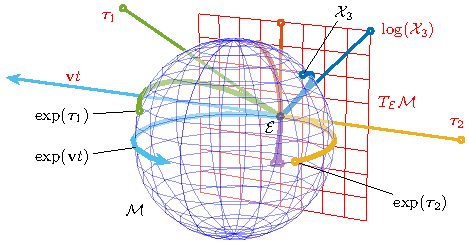
\includegraphics{figures/exponential}
\caption{Lie群与Lie代数关系的表示。
Lie代数 $\mtanat{\cM}{\cE}$ (红色平面)是Lie群流形 $\cM$ (这里用蓝色球面表示)在幺元 $\cE$ 处的切空间。
通过指数映射,每个通过Lie代数原点的直接路径 $\bfv t$ 产生一个围绕流形的路径 $\exp(\bfv t)$ ,流形沿着各自的测地线运行。 
相反的,群中的每个元素在李代数中都有一个等价项。
这种关系是如此深刻,以至于(几乎)群中的所有运算,那些曲线的和非线性的,在李代数中,这是一个线性向量空间,有一个精确的等价。
虽然 $\bbR^3$ 中的球面不是Lie群(我们只是把它当作一个可以画在纸上的表示),但 $\bbR^4$ 中的球面是Lie群,它描述了单位四元数群 --- 参见 \figRef{fig:manifold_q} 和 \exRef{ex:S3} 。
}
\label{fig:exponential}
\end{figure}

当第一次介绍Lie群时,从不同的角度看待它是很重要的。 
拓扑观点,参见 \figRef{fig:exponential} ,涉及流形的形状,并传达其与切空间和指数映射关系的强大直觉。
代数观点涉及群运算及其具体实现,允许利用代数性质来扩展闭式公式或简化它们。
几何视点在机器人学中特别有用,它将群元素与机体或参考坐标系中的位置、速度、方向和/或其它改变相关联。
原始坐标系可以用群的幺元来标识,并且流形上的任意其它点表示某个“局部”坐标系。
借助这些类比,Lie理论的许多数学抽象可以更接近向量空间、几何、运动学和其它更经典领域的直观概念。


Lie理论绝不简单。 
为了掌握Lie理论的最小概念,我们可以参考下面的三个参考文献。 
首先,Abbaspour的 \emph{``Basic Lie theory"}~\cite{ABBASPOUR-2007-Basic_Lie_theory} 有400多页。
也是类似的标题,Howe的 \emph{``Very basic Lie theory"}~\cite{Howe-Basic_Lie} 共有24(稠密的)页,有时被认为是必读的介绍。
最后,更现代、更著名的Stillwell的 \emph{``Naive Lie theory"}~\cite{STILLWELL-08} 共有200多页。
%
由于这些先例被标记为“基本的”、“非常基本的”和“幼稚的”,本文仅 \pageref{LastPage} 页的目的是进一步简化Lie理论 (因此标题中的形容词为 `微型(micro)')。
我们用两种方式来做。
首先,我们从Lie理论中选择一个素材的小子集。这个子集如此之小,以至于它仅仅是探索Lie理论的潜力。 
然而,它对于我们在机器人学中处理的估计问题(例如惯性预积分、里程计和SLAM、视觉伺服等)中的不确定性管理似乎非常有用,从而实现优化的优雅和严格的设计。
第二,我们用教学的方式来解释它,用大量的冗余来减少进入Lie理论的鸿沟,我们认为这仍然是必需的。
也就是说,我们坚持朝着这个方向努力,命名一个范例标题,Stillwell的文献 \cite{STILLWELL-08},并提供一个更简化的版本。
虽然我们试图将抽象级别保持在最低限度,但正文主体是通用的。
当应用到已知的群(旋转和运动矩阵、四元数等)时,插入的示例作为一般概念的基础。 
此外,许多标题非常冗长的插图再次解释了相同的概念。
我们特别关注Jacobian矩阵的计算 (这是一个在文献 \cite{STILLWELL-08} 中没有讨论的主题),它是大多数优化算法的关键,也是设计新算法时的麻烦源。
我们在最后一章给出了机器人定位和映射的应用实例,并在Lie理论基础上实现了EKF和非线性优化算法。
最后,几个附录包含了机器人学中最常用群最相关的详细信息:单位复数、四元数、二维和三维旋转矩阵、二维和三维刚体运动矩阵以及平凡平移群。


然而,我们对Lie理论最重要的简化是在范围方面。 
下面来自 
Howe~\cite{Howe-Basic_Lie} 的一段话可以帮助我们说明我们留下的东西:
%
``\emph{Lie理论的本质现象是人们可以用一种自然的方式联想到Lie群 $\cG$ 和它的Lie代数 $\frak{g}$。
Lie代数 $\frak{g}$ 首先是一个向量空间,其次被赋予一个称为Lie括号 [...] 的双线性非关联积。 
令人惊奇的是,群 $\cG$ 几乎完全由 $\frak{g}$ 和它的Lie括号决定。
因此,对于许多用途,可以用 $\frak{g}$ 代替 $\cG$。
因为 $\cG$ 是一个复杂的非线性对象,而 $\frak{g}$ 只是一个向量空间,所以使用 $\frak{g}$ 通常非常简单。
[...] 
这是Lie理论的力量源泉之一。%
}"
%
在文献 \cite{STILLWELL-08},Stillwell 甚至称为 ``\emph{Lie理论的奇迹}''.
在本次工作中,我们将有效地将Lie代数降级到第二平面,以支持它的等价向量空间 $\bbR^n$,因而根本不引入Lie括号。
因此,Lie群和它的Lie代数之间的联系在这里将不会像它应有的那样深刻。
我们的立场是,鉴于我们所预见的目标应用领域,这种(包含Lie括号的)素材通常是没有必要的。
%). 
此外,如果包含Lie括号在内,那么我们将无法达到清晰和有用的目标,因为读者将不得不进入数学概念,这些概念由于其抽象性或微妙性而变得不必要的复杂。



我们的努力与最近关于这个主题 ~\cite{BARFOOT-17-Estimation,EADE-Lie,forster2017-TRO} 的其它工作是一致的,这些工作也显示了带入Lie理论更进入机器人的需求。
我们的方法旨在让本文的目标读者,熟悉状态估计(Kalman滤波、基于图的优化等),但还不熟悉Lie理论的理论文献的读者,熟悉该理论。
%
为此,我们在符号方面采取了一些倡议,特别是在导数的定义方面,使其接近向量对应项,从而使链式规则清晰可见。
如前所述,我们实际上选择了避免Lie代数的素材,而是更喜欢研究它的同构切向量空间 $\bbR^n$,这是我们最终表示不确定性或(小)状态增量的地方。
所有这些步骤都是在绝对没有精度或准确性损失的情况下进行的,我们相信它们使得理解Lie理论及其工具的操作更容易。

本文伴随一个新的开源的只有头文件的 C++ 代码库,称为 \manif\ \cite{DERAY-20-manif},可以在这里找到: \url{https://github.com/artivis/manif} 。
\manif\ 实现广泛使用的群 $\SO(2)$, $\SO(3)$, $\SE(2)$ 和 $\SE(3)$,并支持创建分析 Jacobian 矩阵。
该库为易于使用、灵活性和性能而设计。


% !TEX root = micro_Lie_theory.tex

\section{微型 Lie 理论}

 
%%%%%%%%%%%%%%%%%%%%%%%%%%%%%%%%%%%%%%%%%%%%%%%%%%%%%%%%%%%%%%%%%
\subsection{Lie 群}

\begin{figure}[tb]
\centering
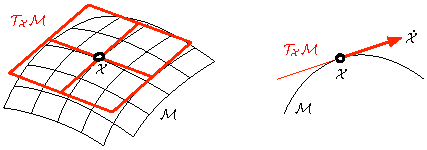
\includegraphics{figures/manifold_tg}
\caption{一个流形 $\cM$ 和向量空间 $\mtanat{\cM}{\cX}$ (在这种情况下 $\cong\bbR^2$)在 $\cX$ 点正切,并有方便的侧切。速度元素, $\dot\cX=\dparil{\cX}{t}$ ,不属于流形 $\cM$ ,但属于切空间 $\mtanat{\cM}{\cX}$。}
\label{fig:manifold_tg}
\end{figure}





在一个唯一的机体中 Lie 群包含群(\emph{group})和光滑流形(\emph{smooth manifold})的概念:Lie群 $\cG$ 是一个光滑流形,其元素满足群公理。
在将这两个概念结合在一起之前,我们将简要介绍这两个概念。

一方面,可微或光滑流形(\emph{smooth manifold})是局部类似于线性空间的拓扑空间。
读者应该能够形象地理解多方面的思想(\figRef{fig:manifold_tg}):它就像一个弯曲的、光滑的(超)表面,没有边缘或尖刺,嵌入到更高维度的空间中。
在机器人学中,我们说我们的状态向量是在这个曲面上演化的,也就是说,流形描述了或是由施加在状态上的约束来定义的。
例如,具有单位范数约束的向量定义半径为$1$的球面流形。
流形的光滑性意味着在每个点上存在唯一的切空间。
这个空间是一个线性或向量空间,我们可以在上面做微积分。 


另一方面,
一个群(\emph{group} $(\cG,\circ)$)是一个集合, $\cG$,具有组合运算, $\circ$,这个算子,对于元素 $\cX,\cY,\cZ\in \cG$,满足下列公理,
%
\begin{align}
\textrm{封闭于 `$\circ$'} & ~:~~ \cX\circ \cY \in \cG  \label{equ:axiom_composition}      \\ 
\textrm{幺元 $\cE$}     & ~:~~ \cE\circ \cX = \cX\circ \cE=\cX  \label{equ:axiom_identity}    \\
\textrm{逆元 $\cX\inv$}    & ~:~~ \cX\inv\circ \cX=\cX\circ \cX\inv=\cE \label{equ:axiom_inverse} \\
\textrm{结合性}      & ~:~~ (\cX\circ \cY)\circ \cZ=\cX\circ(\cY\circ \cZ) 
~.
\end{align}
%


在一个Lie群(\emph{Lie group})中,流形在每一点上看起来都是一样的(例如在球面的表面上,参见 Exs.~\ref{ex:S1} 和 \ref{ex:S3_intro}),并且因此在任何点上的所有切空间都是相同的。 
群结构要求流形元素的组合保持在流形上,方程\eqRef{equ:axiom_composition},并且每个元素在流形中也有一个逆元,方程\eqRef{equ:axiom_inverse}。
其中一个特别的元素是幺元,方程\eqRef{equ:axiom_identity},并因此有一个特殊的切空间是幺元处的正切,我们称之为Lie群的Lie代数。
Lie群结合了光滑流形的局部性质,使我们能够利用群的全局性质进行微积分,从而实现远处对象的非线性组合。

% 在本项工作中,为了简单起见,并且在机器人学工作中很常见,我们经常将Lie群称为“流形”。

%
%
\begin{figure}[tb]
\centering
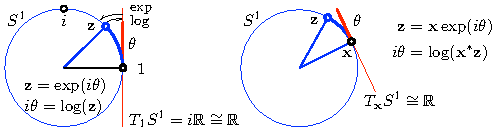
\includegraphics{figures/manifold_z}
\caption{$S^1$ 流形是平面 $\bbC$ 中的单位圆(蓝色),单位复数 $\bfz^*\bfz=1$ 驻留其中。 
Lie代数 $\frak{s}^1=\mtanat{S^1}{\cE}$ 是虚数的线 $i\bbR$ (红色),任何切空间 $\mtan{S^1}$ 都与线 $\bbR$ (红色)同构。
切线向量(红色线段)缠绕流形,形成圆的弧段(蓝色弧段)。
映射 $\exp$ 和 $\log$ 将 $i\bbR$ 的元素(箭头)映射(缠绕和展开)到/自 $S^1$ (蓝色弧段)的元素。
单位复数之间的增量通过组合与指数映射在切线空间中表示(并且我们将为此定义特殊算子 $\op,\om$)。
请参阅正文,以及 \figRef{fig:manifold_q} 所阐述的一个相似的群。
}
\label{fig:manifold_z}
\end{figure}
%

\if\examples y
% !TEX root = micro_Lie_theory.tex


%%%%%%%%%%%%%%%%%%%%%%%%%%%%%  S1  %%%%%%%%%%%%%%%%%%%%%%%%%%%%%%%%
\begin{fexample}	{单位复数群 $S^1$}
\label{ex:S1}

我们的第一个Lie群的例子,是最容易可视化的,是复数乘法下的单位复数群 (\figRef{fig:manifold_z})。
单位复数的形式 $\bfz=\cos\theta+i\sin\theta$。

\emph{-- 作用:}
向量 $\bfx=x+iy$ 在平面内通过复数乘法 $\bfx'=\bfz\,\bfx$ 旋转一个角度 $\theta$。

\emph{-- 群事实:}
单位复数的乘积为单位复数,幺元为 $1$,并且逆元是共轭 $\bfz^*$。

\emph{-- 流形事实:} 
单位范数约束定义了复平面中的单位圆(可以将其视为一维球面,因此命名为 $S^1$)。
这是二维空间中的 1-DoF 曲线。 
单位复数在这个圆上随时间演化。
该群(该圆)在局部重新组装线性空间(切线),而不是在全局重新组装。
\end{fexample}
%%%%%%%%%%%%%%%%%%%%%%%%%%%%%%%%%%%%%%%%%%%%%%%%%%%%%%%%%%%%%%%%%

\fi

\begin{figure}[t]
\centering
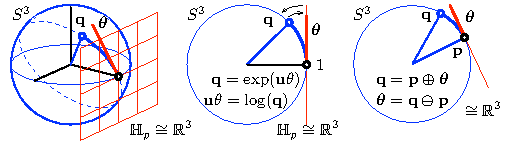
\includegraphics{figures/manifold_q}
\caption{$S^3$ 流形是四元数 $\bbH$ 的四维空间中的单位三维球面(蓝色),单位四元数 $\bfq^*\,\bfq=1$ 驻留其中。
Lie代数是纯虚四元数 $ix+jy+kz\in\bbH_p$ 的空间,同构于超平面 $\bbR^3$ (红色网格),任何其它切空间 $\mtan{S^3}$ 也同构于 $\bbR^3$。
切向量(红色线段)将流形缠绕在大圆弧或测地线(\emph{geodesic})(虚线)上。
中间和右边的图显示了通过该测地线的一个侧切(请注意它与 \figRef{fig:manifold_z} 中的 $S^1$ 有多么相似)。
映射 $\exp$ 和 $\log$ 将 $\bbH_p$ 的元素(箭头)映射(缠绕和展开)到/自 $S^3$ (蓝色弧段)的元素。
四元数之间的增量通过算子 $\op,\om$ 在切空间中表示(参见正文)。
}
\label{fig:manifold_q}
\end{figure}
%
\if\examples y
% !TEX root = micro_Lie_theory.tex

%%%%%%%%%%%%%%%%%%%%%%%%%%%%%  S3  %%%%%%%%%%%%%%%%%%%%%%%%%%%%%%%%
\begin{fexample}	{单位四元数群 $S^3$}
\label{ex:S3_intro}
Lie群的第二个例子,也相对容易可视化,是四元数乘法下的单位四元数群 (\figRef{fig:manifold_q})。
单位四元数的形式 $\bfq=\cos(\theta/2)+\bfu\sin(\theta/2)$,其中 $\bfu=iu_x+ju_y+ku_z$ 是一个单位旋转轴,并且 $\theta$ 是一个旋转角度。

\emph{-- 作用:}
向量 $\bfx=ix+jy+kz$ 在三维空间中通过双四元数乘积 $\bfx'=\bfq\,\bfx\,\bfq^*$ 围绕单位旋转轴 $\bfu$ 旋转一个角度 $\theta$ 。

\emph{-- 群事实:} 
单位四元数的乘积是单位四元数,幺元为 $1$,并且逆元是共轭 $\bfq^*$。

\emph{-- 流形事实:} 
单位范数约束定义了三维球面 $S^3$,一个球形的三维曲面或4维空间中的流形(\emph{manifold})。
在这个曲面上,单位四元数随时间而演变。
该群(该球面)在局部重新组装线性空间(切超平面 $\bbR^3\subset\bbR^4$),而不是在全局重新组装。
\end{fexample}
%%%%%%%%%%%%%%%%%%%%%%%%%%%%%%%%%%%%%%%%%%%%%%%%%%%%%%%%%%%%%

\fi



%%%%%%%%%%%%%%%%%%%%%%%%%%%%%%%%%%%%%%%%%%%%%%%%%%%%%%%%%%%%%%%%%
\subsection{群作用}

重要的是,Lie群具有变换其它集合元素的能力,产生例如旋转、平移、缩放以及它们的组合。 
它们广泛应用于机器人技术中,包括二维和三维。

给定一个Lie群 $\cM$ 和一个集合 $\cV$,我们注意到 $\cX\cdot v$ 是 $v\in\cV$ 上的 $\cX\in\cM$ 的作用($\emph{action}$),
%
\begin{align}
\cdot~:~\cM\times\cV\to\cV~;~ (\cX,v)\mapsto\cX\cdot v
~.
\end{align}
%
对于 $\cdot$ 要成为一个群作用,它必须满足公理, 
%
\begin{align}\label{equ:action}
\textrm{幺元} &:& \cE\cdot v &= v \\
\textrm{相容性} &:& (\cX\circ\cY)\cdot v &= \cX\cdot(\cY\cdot v)
~.
\end{align}


常见的例子有旋转矩阵群 $\SO(n)$,单位四元数群和刚体运动群 $\SE(n)$。
它们各自对向量的作用满足
%
\begin{align*}
\SO(n) &:\textrm{旋转矩阵 } & \bfR\cdot\bfx &\te \bfR\bfx \\
\SE(n) &:\textrm{欧氏矩阵 } & \bfH\cdot\bfx &\te \bfR\bfx + \bft \\
S^1  &:\textrm{单位复数 } & \bfz\cdot\bfx &\te \bfz\,\bfx \\
S^3  &:\textrm{单位四元数 } & \bfq\cdot\bfx &\te \bfq\,\bfx\,\bfq^*
\end{align*}
%
对于更详细的阐述,参见 \tabRef{tab:manifolds} ,以及附录的内容。

% !TEX root = micro_Lie_theory.tex

\begin{table*}[tb]
\caption{二维和三维运动中使用的经典Lie群,包括平凡的 $\bbR^n$。完整参考见附录 
%and the IMU delta composite
}
\label{tab:manifolds}
\begin{center}
\begin{tabular}{|c|c|c|c|c|c|c|c|c|c|c|}
\multicolumn{2}{|c|}{Lie群 $\cM,\circ$} & \!大小\! & \!维度\! 
  & $\cX\in\cM$ 
  & 约束
  & $\bftau^\wedge\in\frak{m}$    
  & $\bftau\in\bbR^m$ 
  & $\Exp(\bftau)$  
  & 组合
  & 作用
  \\
\toprule
%& R^n  ----------------------      
$n$维向量  & $\bbR^n,+$ & $n$  & $n$ 
  & $\bfv\in\bbR^n$ 
  & $\bfv-\bfv=\bf0$
  & $\bfv\in\bbR^n$     
  & $\bfv\in\bbR^n$  
  & $\bfv=\exp(\bfv)$ 
  & $\bfv_1\!+\!\bfv_2$
  & $\bfv + \bfx$
  \\
\midrule
%& S1   ----------------------
圆        & $S^1,\cdot$   & 2    & 1 
  & $\bfz\in\bbC$ 
  & $\bfz^*\bfz=1$
  & $i\theta\in i\bbR$  
  & $\theta\in\bbR$  
  & $\bfz=\exp(i\theta)$ 
  & $\bfz_1\,\bfz_2$
  & $\bfz\,\bfx$
  \\
%& SO(2) ---------------------
旋转   & $\SO(2),\cdot$ & 4    & 1 
  & $\bfR$ 
  & $\bfR\tr\bfR=\bfI$
  & $\hatx{\theta}\in\so(2)$     
  & $\theta\in\bbR$    
  & $\bfR=\exp(\hatx{\theta})$ 
  & $\bfR_1\,\bfR_2$
  & $\bfR\,\bfx$
  \\
%& SE(2)  -------------------- 
刚体运动  
  & $\SE(2),\cdot$ & 9    & 3   
  & $\bfM=\begin{bsmallmatrix}\bfR & \bft \\ 0 & 1\end{bsmallmatrix}$ 
  & $\bfR\tr\bfR=\bfI$
  & $\begin{bsmallmatrix}\hatx{\theta} & \bfrho \\ 0 & 0 \end{bsmallmatrix} \!\in\!\se(2)$     
  & $\begin{bsmallmatrix}\bfrho\\ \theta\end{bsmallmatrix}\in\bbR^3$  
  & $\exp\left(\begin{bsmallmatrix}\hatx{\theta} & \bfrho \\ 0 & 0\end{bsmallmatrix}\right)$ 
  & $\bfM_1\,\bfM_2$
  & $\bfR\,\bfx\!+\!\bft$
  \\
\midrule
%& S3  -----------------------  
三维球面      & $S^3,\cdot$ & 4    & 3   
  & $\bfq\in\bbH$ 
  & $\bfq^*\bfq=1$
  & $\bth/2\in\bbH_p$  
  & $\bth\in\bbR^3$  
  & $\bfq=\exp(\bfu\theta/2)$ 
  & $\bfq_1\,\bfq_2$
  & $\bfq\,\bfx\,\bfq^*$ 
  \\
%& SO(3) ---------------------
旋转   & $\SO(3),\cdot$ & 9    & 3   
  & $\bfR$ 
  & $\bfR\tr\bfR=\bfI$
  & $\hatx{\bth}\in\so(3)$     
  & $\bth\in\bbR^3$  
  & $\bfR=\exp(\hatx{\bth})$ 
  & $\bfR_1\,\bfR_2$
  & $\bfR\,\bfx$
  \\
%& SE(3)  -------------------- 
刚体运动  & $\SE(3),\cdot$   & 16   & 6 
  & $\bfM=\begin{bsmallmatrix}\bfR & \bft \\ 0 & 1\end{bsmallmatrix}$ 
  & $\bfR\tr\bfR=\bfI$
  & $\begin{bsmallmatrix}\hatx{\bth} & \bfrho \\ 0 & 0\end{bsmallmatrix} \!\in\!\se(3)$     
  & $\begin{bsmallmatrix}\bfrho\\\bth\end{bsmallmatrix}\in\bbR^6$  
  & $\exp\left(\begin{bsmallmatrix}\hatx{\bth} & \bfrho \\ 0 & 0\end{bsmallmatrix}\right)$ 
  & $\bfM_1\,\bfM_2$
  & $\bfR\,\bfx\!+\!\bft$
  \\
%\midrule
%% IMU deltas -----------------
%IMU delta     & $\cD,\boxplus$ & 11    & 10 
%  & $\D=\begin{bsmallmatrix}\Dp\\	\Dq \\ \Dv \\ \Dt \end{bsmallmatrix}$ 
%  & $\!\Dq^*\!\Dq\!=\!1\!$
%  & $\begin{bsmallmatrix}\Dp\\	\bfu\Delta\theta/2 \\ \Dv \\ \Dt \end{bsmallmatrix}$ 
%  & $\begin{bsmallmatrix}\Dp\\	\Dth \\ \Dv \\ \Dt \end{bsmallmatrix}\!\in\!\bbR^{10}$  
%  & $\begin{bsmallmatrix}\Dp\\	\exp(\bfu\Dth/2) \\ \Dv \\ \Dt \end{bsmallmatrix}$ 
%  & $\D_1\!\boxplus\!\D_2$
%  & \textrm{---}
%  \\
\bottomrule
\end{tabular}
\end{center}
\end{table*}%



群的组合方程 \eqRef{equ:axiom_composition} 可能被视为群对自身的操作,$\circ:\cM\times\cM\to\cM$。
另一个有趣的作用是伴随作用(\emph{adjoint action}),我们将在 \secRef{sec:adjoint} 看到它。





%%%%%%%%%%%%%%%%%%%%%%%%%%%%%%%%%%%%%%%%%%%%%%%%%%%%%%%%%%%%%%%%%
\subsection{切空间与Lie代数}

给定 $\cX(t)$ 为在Lie群流形 $\cM$ 上移动的点,它的速度 $\dot\cX=\dparil{\cX}{t}$ 属于 $\cX$ 处与 $\cM$ 正切的空间 (\figRef{fig:manifold_tg}),
我们标记为 $\mtanat{\cM}{\cX}$。
流形的光滑性,即没有边或尖峰,意味着在每个点上存在唯一的切空间。
这种切空间的结构在任何地方都是相同的。





%===============================================================
\subsubsection[The Lie algebra]{Lie代数 $\frak{m}$}

幺元 $\mtanat{\cM}{\cE}$ 处的切空间称为 $\cM$ 的Lie代数(\emph{Lie algebra}),标记为 $\frak{m}$,
%
\begin{align}
\textrm{Lie algebra}&:&\frak{m} &\te \mtanat{\cM}{\cE}~.
\end{align}
%
每一个Lie群都有一个关联的Lie代数。
我们通过以下事实 ~\cite{EADE-Lie} 将Lie群与其Lie代数联系起来(参见 Figs.~\ref{fig:exponential} 和 \ref{fig:maps}):
\begin{itemize}
\item
Lie代数 $\frak{m}$ 是一个向量空间。\footnotemark\ 
因此,它的元素可以用 $\bbR^m$ 中的向量来标识(\emph{identified}),其维数 $m$ 是 $\cM$ 的自由度。
\footnotetext{%
在任意Lie代数中,向量空间被赋予一个称为Lie括号的非结合积。在本项工作中,我们不会利用它。}
\item
指数映射(\emph{exponential map}), $\exp:\frak{m}\to\cM$,将Lie代数的元素精确地转化为群的元素。对数映射是逆操作。
\item
通过线性变换, $\cX$ 处的切空间的向量可以变换到幺元 $\cE$ 处的切空间。这种变换称为伴随(\emph{adjoint})变换。
\end{itemize}
%
%


\begin{figure}[tb]
\centering
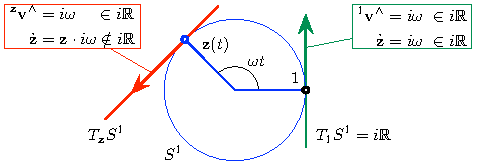
\includegraphics{figures/lie_algebra_S1}
\caption{%
令一个点 $\bfz\in S^1$ 以恒定转速 $\omega$ 移动, $\bfz(t)=\cos\omega t+i\sin\omega t$。
它通过 $1$ 和 $\bfz$ 时的速度分别在 $\mtanat{S^1}{1}$ 和 $\mtanat{S^1}{\bfz}$ 的切空间中。
在 $\mtanat{S^1}{\bfz}$ 的情况下,速度是 $\dot\bfz=\bfz \,i\omega = -\omega\sin\omega t + i\omega\cos\omega t$ 当在全局坐标系中表示时, 并且 ${^\bfz}\!\bfv\hhat=i\omega$ 当在局部表示时。
它们之间的关系为 ${^\bfz}\!\bfv\hhat=\bfz\inv\dot\bfz=\bfz^*\dot\bfz$。
在 $\mtanat{S^1}{1}$ 的情况下,这个关系就是幺元 ${^1}\!\bfv\hhat=\dot\bfz=i\omega$。
显然,所有切空间的结构都是 $i\bbR$,这是Lie代数。
这也是 $\dot\bfz$ 在幺元处的结构,这就是为什么Lie代数被定义为幺元的切空间。
}
\label{fig:global_local_tangent}
\end{figure}


Lie代数可以局部定义到一个切点 $\cX$,建立局部坐标系于 $\mtanat{\cM}{\cX}$
(\figRef{fig:global_local_tangent})。
我们将用“帽子”修饰符来表示Lie代数的元素,例如 $\bfv\hhat$ 表示速度或 $\bftau\hhat=(\bfv t)\hhat=\bfv\hhat t$ 表示一般元素。
还可以添加一个左上标来指定精确的切空间,例如 ${^\cX}\!\bfv\hhat\in\mtanat{\cM}{\cX}$ 和 ${^\cE}\!\bfv\hhat\in\mtanat{\cM}{\cE}$。



通过对群约束方程~\eqRef{equ:axiom_inverse}进行时间微分,Lie代数的结构可以在这里%
%
\if \examples y (参见 Examples~\ref{ex:SO3} 和 \ref{ex:S3}) \else \fi 
%
被找到。
对于乘法群,这将产生新的约束 $\cX\inv\dot\cX + \dot{\cX\inv}\cX = 0$,适用于正切于 $\cX$ 的元素(项 $\dot{\cX\inv}$ 是逆项的导数) 。
因此,Lie代数的元素的形式是,\footnote{对于加法李群,约束 $\cX-\cX=0$ 区别于 $\dot\cX=\dot\cX$,也就是说,没有约束影响切空间。这意味着切空间与群空间相同。更多细节请参见 \appRef{sec:Tn} 。}
%
\begin{align}\label{equ:tangent_structure}
\bfv\hhat = \cX\inv\dot\cX &= -\dot{\cX\inv}\cX
~.
\end{align}
%



%===============================================================
\subsubsection[The Cartesian vector space]{笛卡尔向量空间 $\bbR^m$}

\begin{figure}[tb]
\centering
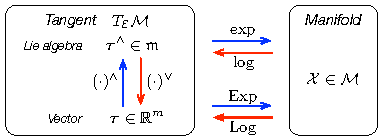
\includegraphics{figures/maps}
\caption{流形 $\cM$ 与其原点 $\mtanat{\cM}{\cE}$ 处的切空间的表示之间的映射(Lie代数 $\frak{m}$ 和笛卡尔 $\bbR^m$)。
映射 hat $(\cdot)\hhat$ 和 vee $(\cdot)\vvee$ 是线性可逆映射或同构(\emph{isomorphisms})方程\eqsRef{equ:hat}{equ:vee},$\exp(\cdot)$ 和 $\log(\cdot)$ 映射 Lie 代数到/自流形,并且 $\Exp(\cdot)$ 和 $\Log(\cdot)$ 是直接将向量空间 $\bbR^m$ 映射到/自 $\cM$ 的快捷方式。}%
\label{fig:maps}%
\end{figure}%


%
Lie代数的元素 $\bftau\hhat$ 具有非平凡结构(斜对称矩阵、虚数、纯虚四元数,参见 \tabRef{tab:manifolds}),
但对我们来说,关键的方面是,它们可以表示为一些基本元素 $E_i$ 的线性组合,其中 $E_i$ 被称为 $\frak{m}$ 的生成元(\emph{generators}) 
(它们是 $\cX$ 在第 $i$ 个方向上围绕原点的导数)。
在 $\bbR^m$ 中将坐标作为向量进行操作是很方便的,我们简单地标记为 $\bftau$。
我们可以从 $\frak{m}$ 传递到 $\bbR^m$ ,反之亦然,通过两个相互逆的线性映射或同构(\emph{isomorphisms}),通常称为 \emph{hat} 和 \emph{vee} (参见 \figRef{fig:maps}),
%
\begin{align} 
\textrm{Hat}&:& 
\bbR^m&\to\frak{m}\,; 
 & 
 \bftau\,
 &\mapsto \bftau\hhat 
 = \sum_{i=1}^m \tau_i\, E_i \label{equ:hat} 
\\
\textrm{Vee}&:& 
 \frak{m}&\to\bbR^m\,; 
 & \bftau\hhat
 & \mapsto (\bftau\hhat)\vvee
 =\bftau
 = \sum_{i=1}^m \tau_i\,\bfe_i  \label{equ:vee}
~,
\end{align}
%
其中 $\bfe_i$ 是 $\bbR^m$ 的基向量(我们有 $\bfe_i\hhat=E_i$)。
这意味着 $\frak{m}$ 与向量空间 $\bbR^m$ 同构 
--- 一个写为 $\frak{m}\cong\bbR^m$, 或者 $\bftau\hhat\cong\bftau$。
对于我们的意图来说,向量 $\bftau\in\bbR^m$ 比它们的同构 $\bftau\hhat\in\frak{m}$ 更易使用,因为它们可以堆叠在更大的状态向量中,更重要的是,可以使用矩阵算子用线性代数进行操作。
在本项工作中,我们实施了 $\bbR^m$ 优于 $\frak{m}$ 的偏好,以至于我们定义的大多数算子和对象(特别是:伴随、Jacobian、扰动及其协方差矩阵,我们很快就会看到)都在 $\bbR^m$ 之上。



\if\examples y
% !TEX root = micro_Lie_theory.tex

%%%%%%%%%%%%%%%%%%%%%%%%%%% SO3 %%%%%%%%%%%%%%%%%%%%%%%%%%%%%%%%%%
\begin{fexample}{旋转群 $\SO(3)$, 它的 Lie 代数 $\so(3)$, 及其向量空间 $\bbR^3$}
\label{ex:SO3}
在 $3\tcross3$ 旋转矩阵 $\bfR$ 的旋转群 $\SO(3)$ 中,我们有正交条件 $\bfR\tr\bfR=\bfI$。
切空间可以通过取该约束的时间导数来找到,即 $\bfR\tr\dot\bfR+\dot\bfR\tr\bfR=0$,我们将其重新排列为 $$\bfR\tr\dot\bfR=-(\bfR\tr\dot\bfR)\tr.$$
这个表达式表明 $\bfR\tr\dot\bfR$ 是一个斜对称矩阵(其转置的负数)。
斜对称矩阵通常用 $\hatx{\bw}$ 表示,其形式如下 
%
$$\hatx{\bw}=\begin{bsmallmatrix}
0 & -\omega_z & \omega_y \\
\omega_z & 0 & -\omega_x \\
-\omega_y & \omega_x & 0 
\end{bsmallmatrix}
.$$
%
这给出 $\bfR\tr\dot\bfR=\hatx{\bw}$。当 $\bfR=\bfI$ 我们有 $$\dot\bfR=\hatx{\bw},$$ 也就是说 $\hatx{\bw}$ 在 $\SO(3)$ 的Lie代数中,我们称之为 $\so(3)$。
%
由于 $\hatx{\bw}\in\so(3)$ 有 $3$ 个自由度, $\SO(3)$ 的维数是 $m=3$。
Lie代数是一个向量空间,它的元素可以分解为
%
$$
\hatx{\bw} = 
  \omega_x\bfE_x+
  \omega_y\bfE_y+
  \omega_z\bfE_z
$$
其中  
$
\bfE_x=
\begin{bsmallmatrix}0&0&0\\0&0&-1\\0&1&0\end{bsmallmatrix}$, 
$\bfE_y=
\begin{bsmallmatrix}0&0&1\\0&0&0\\-1&0&0\end{bsmallmatrix}$,
 $\bfE_z=
\begin{bsmallmatrix}0&-1&0\\1&0&0\\0&0&0\end{bsmallmatrix}$ 
为 $\so(3)$ 的生成元,并且其中 $\bw=(\omega_x,\omega_y,\omega_z)\in\bbR^3$ 是角速度向量。 
%
上面的一对一线性关系允许我们用 $\bbR^3$ 标识 $\so(3)$ --- 我们写为 $\so(3)\cong\bbR^3$。
我们使用线性算子 \emph{hat} 和 \emph{vee} 从 $\so(3)$ 传递到 $\bbR^3$ ,反之亦然,
%
\begin{align*}
\textrm{Hat}&:& \bbR^3&\to\so(3);& \bw&\mapsto\bw^\wedge=\hatx{\bw} 
\\
\textrm{Vee}&:& \so(3)&\to\bbR^3;& \hatx{\bw}&\mapsto\hatx{\bw}^\vee=\bw
~.
\end{align*}
\end{fexample}
%%%%%%%%%%%%%%%%%%%%%%%%%%%%%%%%%%%%%%%%%%%%%%%%%%%%%%%%%%%

\fi



%%%%%%%%%%%%%%%%%%%%%%%%%%%%%%%%%%%%%%%%%%%%%%%%%%%%%%%%%%%%%%%%%
\subsection{指数映射}


\if\examples y
% !TEX root = micro_Lie_theory.tex

%%%%%%%%%%%%%%%%%%%%%%%%% SO3 exp %%%%%%%%%%%%%%%%%%%%%%%%%%%%%%
\begin{fexample}{$\SO(3)$ 的指数映射}
\label{ex:SO3_exp}
%
%We derive here an expression for the exponential map,
%%
%\begin{align*}
%\exp : \so(3)&\to\SO(3);\\
%\hatx{\bth}&\mapsto\exp(\hatx{\bth})
%~.
%\end{align*}
%
我们在 \exRef{ex:SO3} 中看到 
$
\dot\bfR = \bfR\hatx{\bfomega}  \in \mtanat{\SO(3)}{\bfR}.
$
%
对于 $\bw$ 常数,这是一个常微分方程(ODE),其解为 $\bfR(t) = \bfR_0\exp(\hatx{\bfomega}t)$。在原点 $\bfR_0=\bfI$ ,我们有指数映射,
%
\begin{align*}
\bfR(t) &= \exp(\hatx{\bfomega}t) && \in\SO(3)
~. 
\end{align*}
%
我们现在将向量 $\bth\te\bfu\theta \te \bfomega t\in\bbR^3$ 定义为角-轴形式的积分旋转,其中角度 $\theta$ 和单位轴 $\bfu$。 
因此, $\hatx{\bth}\in\so(3)$ 是Lie代数中表示的总旋转。
我们用上面的代换它。 
然后把指数写成幂级数,
%
\begin{align*}
\bfR &= \exp(\hatx{\bth})= \sum_k\frac{\theta^k}{k!}{(\hatx{\bfu})^k} 
~.
\end{align*}
%
为了找到一个封闭形式的表达式,我们写下 $\hatx{\bfu}$ 的几次幂,
%
\begin{align*}
\hatx{\bfu}^0&= \bfI,
&
\hatx{\bfu}^1&= \hatx{\bfu},
\\
\hatx{\bfu}^2&= \bfu\bfu\tr -\bfI,
&
\hatx{\bfu}^3&=-\hatx{\bfu},
\\
\hatx{\bfu}^4&=-\hatx{\bfu}^2,
&
\cdots
\end{align*}
%
并意识到,所有这些都可以表示为 $\bfI$、$\hatx{\bfu}$ 或 $\hatx{\bfu}^2$ 的倍数。
因此,我们将这个级数改写为,
%We substitute them in the series, and group the terms according to the nature of the powers, 
%
\begin{align*}
\bfR = \bfI &+ \hatx{\bfu}\big(\theta - \tfrac1{3!}\theta^3 + \tfrac1{5!}\theta^5 - \cdots\big) \\
  &+ \hatx{\bfu}^2\big(\tfrac12\theta^2-\tfrac1{4!}\theta^4+\tfrac1{6!}\theta^6-\cdots\big)
  ~,
\end{align*}
%
其中,我们确定了 $\sin\theta$ 和 $\cos\theta$ 的级数,得到了封闭形式,
%
\begin{align*}
\bfR=\exp(\hatx{\bfu\theta}) &= 
\bfI + \hatx{\bfu}\sin\theta + \hatx{\bfu}^2(1\!-\!\cos\theta)
~.
\end{align*}
%
这个表达式是众所周知的Rodrigues旋转公式。
它可以用作大写指数方程,只需这么操作 $\bfR=\Exp(\bfu\theta)=\exp(\hatx{\bfu\theta})$。
\end{fexample}
%%%%%%%%%%%%%%%%%%%%%%%%%%%%%%%%%%%%%%%%%%%%%%%%%%%%%

\fi

指数映射 $\exp()$ 允许我们精确地将Lie代数的元素变换到群(\figRef{fig:exponential})上,一般称为收回(\emph{retraction})操作。
直观地说, $\exp()$ 将切元素缠绕在大圆弧或测地线(\emph{geodesic})跟随的流形上(就像将弦缠绕在球上一样, Figs.~\ref{fig:exponential}, \ref{fig:manifold_z} 和 \ref{fig:manifold_q})。
反向映射是 $\log()$,即展开操作。
 $\exp()$ 映射通过考虑流形上 $\cX\in\cM$ 的时间导数自然产生,如下所示。
%
从方程 \eqRef{equ:tangent_structure} 我们有,
%
\begin{align}\label{equ:ode}
\dot\cX &= \cX\bfv\hhat 
~.
\end{align}
%
对于 $\bfv$ 为常数,这是一个常微分方程(ODE),其解是 
%
\begin{align}\label{equ:exp_at_X}
\cX(t)  = \cX(0)\exp(\bfv\hhat t)
~.
\end{align}
%
因为 $\cX(t)$ 和 $\cX(0)$ 是群的元素,所以 $\exp(\bfv\hhat t)=\cX(0)\inv\cX(t)$ 也必须在群中,所以 $\exp(\bfv\hhat t)$ 将Lie代数的元素 $\bfv\hhat t$ 映射到群中。
这被称为指数映射(\emph{exponential map})。

为了给指数映射提供一个更通用的定义,让我们定义切增量 $\bftau\te\bfv t\in\bbR^m$ 作为每一时刻的速度,这样我们就有 $\bftau\hhat=\bfv\hhat t\in\frak{m}$ 做为Lie代数中的一个点。
指数映射和它的逆、对数映射,现在可以写成,
%
\begin{align}
\exp &:& \frak{m} & \to\cM      
 &&; & \bftau\hhat &\mapsto \,\cX = \exp(\bftau\hhat) 
 \\
\log &:&     \cM & \to\frak{m} 
 &&; & \cX\,    &\mapsto \bftau\hhat = \log(\cX) ~
~. 
\end{align}


通过写出绝对收敛的泰勒级数,得到了乘法群中指数的封闭形式,
%
\begin{align}
\exp(\bftau\hhat)=\cE+\bftau\hhat+\tfrac12{\bftau\hhat}^2+\tfrac1{3!}{\bftau\hhat}^3+\cdots
~,
\end{align}
%
并且利用 $\bftau\hhat$ 的幂的代数性质%
\if \examples y (对于指数映射在 $\SO(3)$ 和 $S^3$ 中的扩展参见 Ex.~\ref{ex:SO3_exp} 和 \ref{ex:S3})。 \else. \fi
然后将这些求逆以找到对数映射。
%
指数映射的关键性质是 
%
\begin{align}
\exp((t+s)\bftau\hhat) 
 &= \exp(t\bftau\hhat)\exp(s\bftau\hhat) \label{equ:prop_exp_ts}
 \\
\exp(t\bftau\hhat) 
 &= \exp(\bftau\hhat)^t \label{equ:prop_exp_t}
 \\
\exp(-\bftau\hhat) 
 &= \exp(\bftau\hhat)\inv \label{equ:prop_exp_inv}
 \\
\exp(\cX\bftau\hhat\cX\inv) 
 &= \cX\exp(\bftau\hhat)\cX\inv ~, \label{equ:prop_exp}
\end{align} 
%
其中方程 \eqRef{equ:prop_exp},这是一个惊奇而有力的说明,可以通过扩展泰勒级数和简化许多项 $\cX\inv\cX$ 来轻易地证明。

\if\examples y
% !TEX root = micro_Lie_theory.tex

%%%%%%%%%%%%%%%%%%%% S3 cont %%%%%%%%%%%%%%%%%%%%%%%%%%%%%%%%%
\begin{fexample}{单位四元数群 $S^3$ (条件)}
\label{ex:S3}
在 $S^3$ 群中(回想 \exRef{ex:S3_intro} 并参见 \eg\ \cite{SOLA-17-Quaternion}),单位范数条件 $\bfq^*\bfq=1$ 的时间导数产生 
%
$$\bfq^*\dot\bfq=-(\bfq^*\dot\bfq)^*
.
$$
%
这表明 $\bfq^*\dot\bfq$ 是一个纯虚四元数(其实部为零)。
%The set of pure quaternions is noted $\bbH_p$.
纯虚四元数 $\bfu v\in\bbH_p$ 有形式 
%
$$\bfu v=(iu_x+ju_y+ku_z)v =iv_x+jv_y+kv_z 
,$$
%
其中, $\bfu\te iu_x+ju_y+ku_z$ 是纯幺正的, $v$ 是范数,并且 $i,j,k$ 是Lie代数 $\frak{s}^3=\bbH_p$ 的生成元。
%
重写我们上面的条件,
%
\begin{align*}
\dot\bfq=\bfq\, \bfu v &&\in \mtanat{S^3}{\bfq}
,
\end{align*}
% 
那将积分到 $\bfq = \bfq_0\exp(\bfu v t)$。 
令 $\bfq_0=1$ 并定义 $\bphi \te \bfu\phi \te\bfu v t$ 我们得到指数映射,
%
\begin{align*}
\bfq = \exp(\bfu\phi) \te \sum \frac{\phi^k}{k!}\bfu^k &&\in S^3
~.
\end{align*}
%
$\bfu$ 的幂跟随以下模式 $1,\bfu,-1,-\bfu,1,\cdots$。
因此,我们将项分组为 $1$ 和 $\bfu$ ,并标识 $\cos\phi$ 和 $\sin\phi$ 的级数。
我们得到封闭形式,
%
\begin{align*}
\bfq = \exp(\bfu\phi) = \cos(\phi) + \bfu\sin(\phi) 
~,
\end{align*}
%
这是欧拉公式的优美扩展, $\exp(i\phi)=\cos\phi+i\sin\phi$。
%
Lie代数 $\bfphi=\bfu \phi\in\frak{s}^3$ 的元素可以通过映射 \emph{hat} 和 \emph{vee} 用旋转向量 $\bth\in\bbR^3$ 标识,
%
\begin{align*}
\textrm{Hat}&:& \bbR^3&\to\frak{s}^3;& \bth&\mapsto\bth^\wedge=2\bphi
\\
\textrm{Vee}&:& \frak{s}^3&\to\bbR^3;& \bphi&\mapsto\bphi^\vee=\bth/2
~,
\end{align*}
%
其中 %$\bth \te \bfu\theta\te\bw t$ is the angle-axis vector, and 
因子 $2$ 说明了旋转作用中四元数的双重效应, $\bfx'=\bfq\,\bfx\,\bfq^*$。 
%
通过选择 Hat 和 Vee,四元数指数
%
\begin{align*}
\bfq = \Exp(\bfu\theta)=\cos(\theta/2)+\bfu\sin(\theta/2)
\end{align*}
%
等价于旋转矩阵 $\bfR=\Exp(\bfu\theta)$。
\end{fexample}
%%%%%%%%%%%%%%%%%%%%%%%%%%%%%%%%%%%%%%%%%%%%%%%%%%%%%%%%

\fi



%===============================================================
\subsubsection[The capitalized Exp map]{大写指数映射}


大写的 Exp 和 Log 映射是将向量元素 $\bftau\in\bbR^m~(\cong\mtanat{\cM}{\cE})$ 直接映射到元素 $\cX\in\cM$ 的快捷方式。
% 
我们有,
%
\begin{align}
\Exp &: &\bbR^m &\to\cM &&;&
\,\bftau &\mapsto \cX = \Exp(\bftau)\\
\Log  &: & \cM &\to\bbR^m &&;&
 \cX &\mapsto \bftau\,=\Log(\cX) 
\,. 
\end{align}
%
显然来自 \figRef{fig:maps},
%
\begin{align}
\cX  = \Exp(\bftau) &\te \exp(\bftau\hhat) \\
\bftau =\Log(\cX)    &\te \log(\cX)\vvee 
~. 
\end{align}
%
对于不同流形的这些映射的实现的详细信息,参见附录。


%===============================================================
\subsection{加号和减号算子}

加号和减号算子允许我们在(弯曲的)流形的元素之间引入增量,并在(平坦的)切向量空间中表示它们。 
它们用 $\op$ 和 $\om$表示,将一个 Exp/Log 操作与一个结合操作组合在一起。
由于组合的非交换性,它们根据操作数的顺序在右结合(right-)版本和左结合(left-)版本中定义。
右结合(right-)算子是 (参见 \figRef{fig:manifold_q}-\emph{right}), 
%
\begin{align}
\textrm{right-}\op:&& \cY &= \cX\op{^\cX\!\bftau} \te \cX\circ\Exp({^\cX\!\bftau}) \,\in \cM \label{equ:rplus} \\
\textrm{right-}\om:&& {^\cX\!\bftau} &= \cY\om\cX \,\te \Log(\cX\inv\!\circ\!\cY)\in\mtanat{\cM}{\cX} \label{equ:rminus}
~.
\end{align}
%
因为在方程 \eqRef{equ:rplus} 中 $\Exp({^\cX\!\bftau})$ 出现在组合的右手侧,
${^\cX\!\bftau}$ 属于 $\cX$ 处的切空间(参见方程 \eqRef{equ:rminus}): 
我们按照约定\footnotemark~说这个 ${^\cX\!\bftau}$ 是在 $\cX$ 处的局部(\emph{local})坐标系中表示 --- 我们标记到参考坐标系的左上标。

左结合(left-)算子是
\begin{align}
\textrm{left-}\op:&&\cY&={^\cE\!\bftau}\op\cX \te \Exp({^\cE\!\bftau})\circ\cX \in \cM \label{equ:lplus} \\
\textrm{left-}\om:&&{^\cE\!\bftau}&=~\cY\om\cX \te \Log(\cY\!\circ\!\cX\inv)\in\mtanat{\cM}{\cE}
\label{equ:lminus}
~.
\end{align}
%
现在,在方程 \eqRef{equ:lplus} 中 $\Exp({^\cE\!\bftau})$ 在左侧,并且我们有 ${{^\cE\!\bftau}\in\mtanat{\cM}{\cE}}$:我们说这个 ${{^\cE}\!\bftau}$ 是在全局(\emph{global})坐标系中表示。

请注意,虽然右结合(right-)和左结合(left-)算子 $\op$ 是按操作数顺序区分的,但符号 $\om$ 在方程 \eqRef{equ:rminus} 和 \eqRef{equ:lminus} 中是不明确的。
在本项工作中,我们默认表示局部扰动,因此我们默认使用 $\op$ 和 $\om$ 的右结合(right-)形式。
\footnotetext{这个约定坚持坐标系变换,例如${^G\!\bfx=\bfR^L\!\bfx}$,其中 $\bfR\in \SO(3)$ 将局部向量变换为全局向量。
请注意,并非所有作者都共享此约定,例如文献 \cite{GALLEGO-13} 使用了相反的约定, ${^L\!\bfx=\bfR^G\!\bfx}$。}


%===============================================================
\subsection[Adjoint, and adjoint matrix]{伴随和伴随矩阵}
\label{sec:adjoint}

\begin{figure}[tb]
\centering
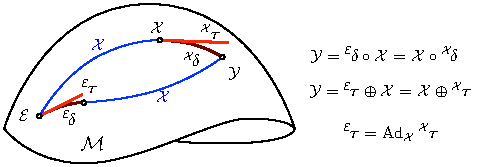
\includegraphics{figures/adjoint}
\caption{两条路径, $\cX\circ{^\cX}\!\delta$ 和 ${^\cE}\!\delta\circ\cX$ ,将原点 $\cE$ 与点 $\cY$ 连接。
它们都用增量或 `deltas' 组成元素 $\cX$ ,在局部坐标系中表示,${^\cX}\!\delta$,或在原点表示, ${^\cE}\!\delta$。
由于非交换性,元素 ${^\cX}\!\delta$ 和 ${^\cE}\!\delta$ 不相等。 
它们的相关切向量 ${^\cX}\!\bftau=\Log({^\cX}\!\delta)$ 和 ${^\cE}\!\bftau=\Log({^\cE}\!\delta)$ 也不相等。
它们联系在一起通过线性变换 ${^\cE}\!\bftau=\Ad[\cM]{\cX}\,{^\cX}\!\bftau$ 其中
$\Ad{\cX}$ 是 $\cM$ 在 $\cX$ 处的伴随。 
}
\label{fig:adjoint}
\end{figure}


如果我们在方程 \eqssRef{equ:rplus,equ:lplus} 中标识 $\cY$ ,我们就得到 ${{^\cE\!\bftau}\op\cX} = {\cX\op{^\cX\!\bftau}}$ ,它确定局部切元素和全局切元素之间的关系 (\figRef{fig:adjoint})。
我们用方程 \eqssRef{equ:prop_exp,equ:rplus,equ:lplus} 来扩展它为
%
\begin{align*}
\Exp({^\cE}\!\bftau)\cX 
 &= \cX\Exp({^\cX}\!\bftau) \\
\exp({^\cE}\!\bftau\hhat) 
 &= \cX \exp({^\cX}\!\bftau\hhat) \cX\inv 
  = \exp(\cX {^\cX}\!\bftau\hhat \cX\inv) \\
{^\cE}\!\bftau\hhat 
 &= \cX {^\cX}\!\bftau\hhat \cX\inv 
\end{align*}
%
\subsubsection{伴随}
因此,我们将 $\cM$ 在 $\cX$ 处的伴随(\emph{adjoint}),记为 $\Adh[\cM]{\cX}$,定义为 
%
\begin{align}
\Adh{\cX}:\frak{m}\to\frak{m};~~ \bftau\hhat\mapsto \Adh[\cM]{\cX}(\bftau\hhat) \te \cX \bftau\hhat \cX\inv \label{equ:Adjh1} 
~,
\end{align}
%
因此 ${^\cE}\!\bftau\hhat = \Adh[\cM]{\cX}({^\cX}\!\bftau\hhat)$。 
这定义了群在它自己的Lie代数上的伴随作用(\emph{adjoint action})。
伴随有两个有趣的(并且很容易证明的)性质,
%
\begin{align*}
\textrm{Linear} &:& \Adh{\cX}(a\bftau\hhat+b\bfsigma\hhat) =& ~a\Adh{\cX}(\bftau\hhat)\\
&&&+b\Adh{\cX}(\bfsigma\hhat) 
\\
\textrm{Homomorphism} &:& \Adh{\cX}(\Adh{\cY}(\bftau\hhat)) =& ~\Adh{\cX\cY}(\bftau\hhat) 
~.
\end{align*}
%
\subsubsection{伴随矩阵}
因为 $\Adh{\cX}()$ 是线性的,我们可以找到一个等价的矩阵算子 $\Ad{\cX}$ ,它映射笛卡尔切向量 ${^\cE}\!\bftau\cong{^\cE}\!\bftau\hhat$ 和 ${^\cX}\!\bftau\cong{^\cX}\!\bftau\hhat$,
%
\begin{align}
\Ad{\cX}:\bbR^m\to\bbR^m;~~ ^\cX\!\bftau\mapsto {^\cE}\!\bftau &= \Ad[\cM]{\cX}{^\cX}\!\bftau \label{equ:Adj2} 
~,
\end{align}
%
我们称之为伴随矩阵(\emph{adjoint matrix})。这可以通过将 $\vvee$ 应用于方程 \eqRef{equ:Adjh1} 来计算,因此写为
%
\begin{align}\label{equ:Adj4} 
\Ad[\cM]{\cX}\,\bftau &= (\cX\bftau\hhat\cX\inv)\vvee 
~,
\end{align}
%
然后扩展右手侧结合以标识伴随矩阵 (参见 Ex.~\ref{ex:SE3_adjoint} 和附录)。
伴随矩阵的其它性质是,
%
\begin{align}
\cX\op\bftau &= (\Ad[\cM]{\cX}\,\bftau)\op\cX \label{equ:Adj1} \\
\Ad[\cM]{\cX\inv} &= \Ad[\cM]{\cX}\inv \label{equ:Adj5} \\
\Ad[\cM]{\cX\cY} &=\Ad[\cM]{\cX}\Ad[\cM]{\cY} \label{equ:Adj7}
~.
\end{align}
%
请注意在方程 \eqssRef{equ:Adj5,equ:Adj7} 中的左半部分通常比右半部分计算起来更便宜。
我们将经常使用伴随矩阵将 $\cX$ 处的切空间的向量线性变换为原点的切空间的向量,使用 ${^\cE}\!\bftau = \Ad{\cX}{^\cX}\!\bftau$ ,方程~\eqRef{equ:Adj2}。
在本项工作中,伴随矩阵将被简单的称为伴随。



\if\examples y
% !TEX root = micro_Lie_theory.tex

%%%%%%%%%%%%%%%%%%%% SE3 adjoint %%%%%%%%%%%%%%%%%%%%%%%%%%%%
\begin{fexample}{$\SE(3)$ 的伴随矩阵}\label{ex:SE3_adjoint}
%
刚体运动的 $\SE(3)$ 群(参见 \appRef{sec:SE3})有群,Lie代数和向量元素,
%
\begin{align*}
\bfM&=\begin{bmatrix}\bfR&\bft\\\bf0&1\end{bmatrix}
~,
&
\bftau\hhat&=\begin{bmatrix}\hatx{\bth}&\bfrho\\\bf0&0\end{bmatrix}
~,
&
\bftau &=\begin{bmatrix}\bfrho\\\bth\end{bmatrix}
~.
\end{align*}
%
伴随矩阵由扩展的方程 \eqRef{equ:Adj4} 标识为
%
\begin{align*}
\Ad{\bfM}\,\bftau
  &= (\bfM\bftau\hhat\bfM\inv)\vvee = \cdots =
  \\
  &= \left(\begin{bmatrix}\bfR\hatx{\bth}\bfR\tr & -\bfR\hatx{\bth}\bfR\tr\bft + \bfR\bfrho \\ \bf0 & \bf0\end{bmatrix}\right)\vvee \\
%  &= \left(\begin{bmatrix}\hatx{\bfR\bth} & -\hatx{\bfR\bth}\bft + \bfR\bfrho \\ \bf0 & \bf0\end{bmatrix}\right)\vvee \\
  &= \left(\begin{bmatrix}\hatx{\bfR\bth} & \hatx{\bft}\bfR\bth + \bfR\bfrho \\ \bf0 & \bf0\end{bmatrix}\right)\vvee \\
  &= \begin{bmatrix}\hatx{\bft}\bfR\bth + \bfR\bfrho \\ \bfR\bth\end{bmatrix} 
%  \\
%  &
  = \begin{bmatrix}\bfR & \hatx{\bft}\bfR\\ \bf0&\bfR\end{bmatrix}\begin{bmatrix}\bfrho \\ \bth\end{bmatrix} 
\end{align*}
%
其中我们使用 $\hatx{\bfR\bth}=\bfR\hatx{\bth}\bfR\tr$ 和 $\hatx{\bfa}\bfb=-\hatx{\bfb}\bfa$ 。所以伴随矩阵是 
%
\begin{align*}
\Ad{\bfM} =  \begin{bmatrix}\bfR & \hatx{\bft}\bfR \\ \bf0&\bfR\end{bmatrix} \quad\in\bbR^{6\times6}
~.
\end{align*}
%
\end{fexample}		
%%%%%%%%%%%%%%%%%%%%%%%%%%%%%%%%%%%%%%%%%%%%%%%%%%%%%%%%%%%%%%%%%

\fi




%%%%%%%%%%%%%%%%%%%%%%%%%%%%%%%%%%%%%%%%%%%%%%%%%%%%%%%%%%%%%%%%%
\subsection{Lie群上的导数}

在Lie群中定义导数的各种方法中,我们主要关注Jacobian矩阵映射向量切空间的形式。 
这在这里就足够了,因为在这些空间中,不确定性和增量可以被恰当而容易地定义。
利用这些Jacobian矩阵,Lie群中的不确定性管理公式与向量空间中的不确定性管理公式基本相似。

下文描述的Jacobian矩阵满足链式规则,因此我们可以很容易地从部分的Jacobian矩阵块的求逆(\emph{inversion})、组合(\emph{composition})、求幂(\emph{exponentiation})和作用(\emph{action})等操作来计算任何Jacobian矩阵。
详情和证明参见 \secRef{sec:jacs_chain_rule} 。


%=======================================================
\subsubsection[Jacobians on vector spaces]{提醒:向量空间上的Jacobian矩阵}

对于多元函数 $f:\bbR^m\to\bbR^n$,Jacobian矩阵定义为所有偏导数的 $n\times m$ 矩阵, 
%
\begin{align}\label{equ:jac_Rn_matrix}
\bfJ = \dpar{f(\bfx)}{\bfx} &\te \begin{bmatrix}
\dpar{f_1}{x_1} & \cdots & \dpar{f_1}{x_m} \\
\vdots && \vdots \\
\dpar{f_n}{x_1} & \cdots & \dpar{f_n}{x_m} 
\end{bmatrix} \in\bbR^{n\times m}
~.
\end{align}
%
用下面的形式定义这个矩阵很方便。让我们分割 $\bfJ=[\bfj_1\cdots\bfj_m]$,并让 $\bfj_i=[\dpar{f_1}{x_i}\cdots\dpar{f_n}{x_i}]\tr$ 作为它的第 $i$ 个列向量。此列向量响应于
%
\begin{align}\label{equ:jac_Rn_i}
\bfj_i = \dpar{f(\bfx)}{x_i} \te \lim_{h\to0}\frac{f(\bfx+h\bfe_i)-f(\bfx)}{h} \in \bbR^n
~,
\end{align}
%
其中 $\bfe_i$ 是 $\bbR^m$ 的自然基的第 $i$ 个向量。
关于分子,注意这个向量 
%
\begin{align}\label{equ:jac_Rn_vec}
\bfv_i(h) \te f(\bfx+h\bfe_i)-f(\bfx) \quad \in\bbR^n
\end{align}
%
是当 $\bfx$ 在 $\bfe_i$ 方向上受到扰动时, $f(\bfx)$ 的变化量,并且相应的Jacobian矩阵的列仅为 $\bfj_i=\dparil{\bfv_i(h)}{h}|_{h=0}=\lim_{h\to0}\bfv_i(h)/h$。
在本项工作中,为了方便起见,我们引入了紧凑形式,
%
\begin{align}\label{equ:jac_Rn}
\mjac{}{}=\dpar{f(\bfx)}{\bfx}\te\lim_{\bfh\to0}\frac{f(\bfx+\bfh)-f(\bfx)}{\bfh}
\in\bbR^{n\times m}
~,
\end{align}
%
其中 $\bfh\in\bbR^m$, 其用方程 \eqRef{equ:jac_Rn_i} 计算所有列
以形成方程 \eqRef{equ:jac_Rn_matrix} 的定义。
我们注意到方程 \eqRef{equ:jac_Rn} 只是一个方便的符号 (就像方程 \eqRef{equ:jac_Rn_matrix} 一样),因为向量 $\bfh$ 的除法未定义,正确的计算需要方程 \eqRef{equ:jac_Rn_i} 。
然而,通过将分子扩展成 $\bfh$ 中的线性形式,并将左手侧标识为Jacobian矩阵,该形式可用于计算Jacobian矩阵,即,
%
\begin{align}\label{equ:jac_Rn_identify}
 \lim_{\bfh\to0}\frac{f(\bfx\!+\!\bfh)\!-\!f(\bfx)}{\bfh} 
 = \cdots
 = \lim_{\bfh\to0}\frac{\bfJ\bfh}{\bfh}  
 \te \dpar{\bfJ\bfh}{\bfh} 
 = \bfJ.
\end{align}
%
最后请注意,对于 $\bfh$ 的小值,我们有线性近似值,
%
\begin{align}
f(\bfx+\bfh) \xrightarrow[\bfh\to0]{} f(\bfx) + \dpar{f(\bfx)}{\bfx}\bfh
~.
\end{align}

%=======================================================
\subsubsection{Lie 群上的右Jacobian矩阵}


\begin{figure}[tb]
\centering
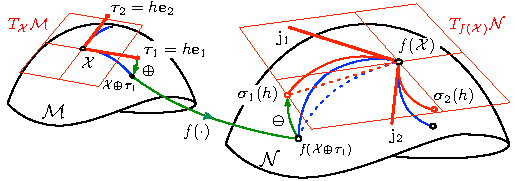
\includegraphics{figures/jacobian}
\caption{函数的右Jacobian矩阵 $f:\cM\to\cN$ 。
正则方向上的扰动向量, $\bftau_i=h\bfe_i\in\mtanat{\cM}{\cX}$,通过加号、应用 $f()$ 和减号(绿色箭头)的过程传播到 $\bfsigma_i\in\mtanat{\cN}{f(\cX)}$ 中的扰动向量,获得 $\bfsigma_i(h)=f(\cX\op h\bfe_i)\om f(\cX)$。 
对于 $h$ 的不同值,请注意,在 $\cM$ 中,扰动 $\bftau_i(h)=h\bfe_i$ (粗红色)沿测地线产生 $\cM$ (蓝色)路径(回忆~\figRef{fig:exponential})。
另请注意,在 $\cN$ 中,由于 $f(\cdot)$ 的非线性,图像路径(蓝色实线)通常不在测地线中(蓝色虚线)。
这些图像路径被提升到切空间 $\mtanat{\cN}{f(\cX)}$,生成平滑的曲线路径(细红色实线)。
$\bfJ$ (粗红线)的列向量 $\bfj_i$ 是在 $f(\cX)$ 处计算的提升路径的导数,
即 $\bfj_i=\lim_{h\to0}\bfsigma_i(h)/h$ 。
每一个 $h\bfe_i\in\mtanat{\cM}{\cX}$ 让位给一个 $\bfj_i\in\mtanat{\cN}{f(\cX)}$,并由此产生的Jacobian矩阵 $\bfJ=[\,\bfj_1\cdots\bfj_m\,]\in\bbR^{n\times m}$ 线性地映射向量从 $\mtanat{\cM}{\cX}\cong\bbR^m$ 到 $\mtanat{\cN}{f(\cX)}\cong\bbR^n$ 。
}
\label{fig:manifold_g}
\end{figure}
%


受上面标准导数定义方程 \eqRef{equ:jac_Rn} 的启发,我们现在可以使用我们的 $\op$ 和 $\om$ 算子来定义作用于流形的函数 $f:\cM\to\cN$ 的Jacobian矩阵(参见 \figRef{fig:manifold_g})。
使用右结合(right-)的 $\{\op,\om\}$ 代替 $\{+,-\}$ 我们获得一个类似于标准导数的形式,\footnote{%
符号 $\ndpar{\cY}{\cX}=\ndpar{f(\cX)}{\cX}$ 在其它替代符号之前被选择,以便使链规则可读,即$\ndpar{\cZ}{\cX}=\ndpar{\cZ}{\cY}\ndpar{\cY}{\cX}$。
稍后我们将介绍更轻量的符号 $\mjac{\cY}{\cX}\te\ndpar{\cY}{\cX}$。
}
%
\begin{subequations}\label{equ:Jacobian_set}
\begin{align}
\rdpar{f(\cX)}{\cX}
&\te \lim_{\bftau\to0}\frac{f(\cX\op\bftau)\om f(\cX)}{\bftau}
~~~~~ \in\bbR^{n\times m} \label{equ:Jacobian} 
\\
\intertext{它扩展为,}
& = \lim_{\bftau\to0}\frac{\Log\big(f(\cX)\inv\circ f(\cX\circ\Exp(\bftau)) \big)}{\bftau} 
 %\notag
\\
&= \pjac{\Log\big(f(\cX)\inv\circ f(\cX\!\circ\!\Exp(\bftau)) \big)}{\bftau}{\bftau=0} 
 \label{equ:Jacobian_aslinear}
.
\end{align}
\end{subequations}
%
我们把这种Jacobian矩阵称为 $f$ 函数的右Jacobian矩阵(\emph{right Jacobian of $f$})。
请注意方程 \eqRef{equ:Jacobian_aslinear} 只是标准导数方程 \eqRef{equ:jac_Rn} 的相当复杂的函数 $g(\bftau)=\Log\big(f(\cX)\inv\circ f(\cX\circ\Exp(\bftau)) \big)$。
将其写入方程 \eqRef{equ:Jacobian} 中传达了更多的直觉:它是 $f(\cX)$ 相对于 $\cX$ 的导数,只是我们表达了切空间中的无穷小变化!
实际上,由于使用右结合(right-)的 $\op$ 和 $\om$ 的操作, $\cX$ 和 $f(\cX)$ 中的变量现在被表示为局部切空间中的向量,即分别在 $\cX\in\cM$ 和 $f(\cX)\in\cN$ 处的正切。
这个导数是一个适当的Jacobian矩阵 $\bbR^{n\times m}$ 线性地映射到局部(\emph{local})切空间 $\mtanat{\cM}{\cX} \to \mtanat{\cN}{f(\cX)}$ (并且我们用一个局部 `$\cX$' 上标来标记导数)。
就像在向量空间中一样,这个矩阵的列对应于方向导数。
也就是向量 
%
\begin{align}
\bfsigma_i(h) &= f(\cX\op h\bfe_i)\om f(\cX) \quad \in\bbR^n \label{equ:jac_N_vec}
\end{align}
%
(再次参见 \figRef{fig:manifold_g} ,并用方程 \eqRef{equ:jac_Rn_vec} 中的 $\bfv_i$ 来比较方程 \eqRef{equ:jac_N_vec} 的 $\bfsigma_i$)
是当 $\cX$ 沿着 $\bfe_i$ 方向变化时, $f(\cX)$ 的变化。
其相应的Jacobian矩阵的列是 $\bfj_i=\dparil{\bfsigma_i(h)}{h}|_{h=0}$。


与前面一样,我们使用方程 \eqRef{equ:Jacobian} 以便使用相同的机制方程 \eqRef{equ:jac_Rn_identify} 来真正地寻找Jacobian矩阵。
%
%
%
例如,对于三维旋转 $f:\SO(3)\to\bbR^3;~f(\bfR)=\bfR\bfp$,我们有 $\cM=\SO(3)$ 和 $\cN=\bbR^3$ ,并因此(参见 \appRef{sec:jac_SO3_action}), 
%
\begin{align*}
\rdpar{\bfR\bfp}{\bfR}
 &= \lim_{\bth\to0}\frac{(\bfR\op\bth)\bfp\om\bfR\bfp}{\bth} 
 = \lim_{\bth\to0}\frac{\bfR\Exp(\bth)\bfp-\bfR\bfp}{\bth} \\
 &= \lim_{\bth\to0}\frac{\bfR(\bfI+\hatx{\bth})\bfp-\bfR\bfp}{\bth} 
 = \lim_{\bth\to0}\frac{\bfR\hatx{\bth}\bfp}{\bth} \\
 &= \lim_{\bth\to0}\frac{-\bfR\hatx{\bfp}\bth}{\bth} 
 = -\bfR\hatx{\bfp} 
 ~~~\in \bbR^{3\times 3}
 ~.
\end{align*}
%
此机制的许多示例可以在 \secRef{sec:derivatives_M} 和附录中看到。
%
备注,每当函数 $f$ 从一个流形传递到另一个流形时,方程 \eqRef{equ:Jacobian} 中的加号和减号算子必须被正确选择:
$\op$ 对应定义域(domain) $\cM$,并且 $\om$ 对应目标域(codomain)或图(image) $\cN$ 。


对于 $\bftau$ 的小值,以下近似值适用,
%
\begin{align}\label{equ:lin_approx}
f(\cX\op{^\cX\!\bftau}) \xrightarrow[{^\cX\!\bftau}\to0]{} f(\cX)\op\rdpar{f(\cX)}{\cX}\,{^\cX\!\bftau}
\quad \in \cN
~.
\end{align}
%



%=======================================================
\subsubsection{Lie 群上的左Jacobian矩阵}

导数也可以由左结合(left-)加号和减号算子定义,从而,
%
\begin{align}\label{equ:left-Jacobian}
\ldpar{f(\cX)}{\cX} 
& \te \lim_{\bftau\to0}\frac{f(\bftau\op\cX)\om f(\cX)}{\bftau}  
~~~~~\in\bbR^{n\times m}
\\
& = \lim_{\bftau\to0}\frac{\Log(f(\Exp(\bftau)\circ\cX) \circ f(\cX)\inv)}{\bftau} \notag
\\
&= \pjac{\Log\big(f(\Exp(\bftau)\circ\cX) \circ f(\cX)\inv\big)}{\bftau}{\bftau=0} \notag
~,
\end{align}
%
我们称之为 $f$ 函数的左Jacobian矩阵(\emph{left Jacobian of $f$})。
请注意,现在 $\bftau\in\mtanat{\cM}{\cE}$,并且分子属于 $\mtanat{\cN}{\cE}$,因此左Jacobian矩阵是一个 $n\times m$ 的矩阵,映射了全局(\emph{global})切空间,$\mtanat{\cM}{\cE}\to\mtanat{\cN}{\cE}$,这是 $\cM$ 和 $\cN$ 的Lie代数(并且我们用全局或原点 `$\cE$' 上标来标记导数)。
对于 $\bftau$ 的小值,以下方程成立,
%
\begin{align}\label{equ:lin_approx_left}
f({^\cE\!\bftau}\op\cX) \xrightarrow[{^\cE\!\bftau}\to0]{} \ldpar{f(\cX)}{\cX}\,{^\cE\!\bftau} \op f(\cX)
\quad \in \cN
~.
\end{align}

\begin{figure}[tb]
\centering
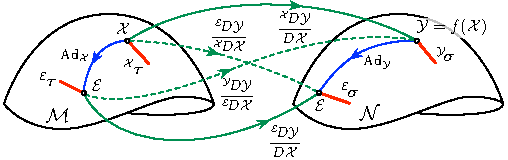
\includegraphics{figures/jacobians_adjoints}
\caption{函数 $\cY=f(\cX)$ 中所有切空间之间的线性映射,从 $\cM$ 到 $\cN$。线性映射 ${{^\cE}\!\bftau=\Ad[\cM]{\cX}\,{^\cX}\!\bftau}$, ${{^\cE}\!\bfsigma=\Ad[\cN]{\cY}\,{^\cY}\!\bfsigma}$, ${{^\cE}\!\bfsigma=\ldpar{\cY}{\cX}\,{^\cE}\!\bftau}$,并且 ${{^\cY}\!\bfsigma=\rdpar{\cY}{\cX}\,{^\cX}\!\bftau}$,形成一个指向方程 \eqRef{equ:derivatives_lr_adjoints} 的循环(实线)。交叉的Jacobian矩阵(虚线)形成了更多的映射循环,导致方程 (\ref{equ:derivatives_ex_adjoints},\ref{equ:derivatives_ye_adjoints})。} 
\label{fig:jacobians_adjoints}
\end{figure}

我们可以从方程 (\ref{equ:Adj1}, \ref{equ:lin_approx}, \ref{equ:lin_approx_left}) (参见 \figRef{fig:jacobians_adjoints}) 中展示左和右Jacobian矩阵由 $\cM$ 和 $\cN$ 的伴随相关联的关系,
%
\begin{align}\label{equ:derivatives_lr_adjoints}
\ldpar{f(\cX)}{\cX}\Ad[\cM]{\cX} = \Ad[\cN]{f(\cX)}\rdpar{f(\cX)}{\cX} 
~.
\end{align}


%=======================================================
\subsubsection{交叉使用右--左Jacobian矩阵}

也可以同时使用右侧加号和左侧减号来定义Jacobian矩阵,反之亦然。
虽然不太可能,但它们有时很有用,因为它们将局部的正切映射到全局的正切,反之亦然。
简而言之,我们将通过伴随把它们与其它Jacobian矩阵联系起来,
%
\begin{align}
\lrdpar{\cY}{\cX} &= \lldpar{\cY}{\cX}\,\Ad{\cX} ~~~\,= \Ad{\cY}\,\rrdpar{\cY}{\cX} \label{equ:derivatives_ex_adjoints}\\
\rldpar{\cY}{\cX} &= \rrdpar{\cY}{\cX}\,\Ad{\cX}\inv = \Ad{\cY}\inv\,\lldpar{\cY}{\cX}\label{equ:derivatives_ye_adjoints}
~,
\end{align}
%
其中 $\cY=f(\cX)$ 。现在,上一行和下一行的上标表明表示差异的参考坐标系。
相应的小 $\bftau$ 的近似值取为,
%
\begin{align}
f(\cX\op{^\cX}\bftau) 
 &\xrightarrow[{^\cX\!\bftau}\to0]{} \lrdpar{f(\cX)}{\cX}\,{^\cX}\bftau \op f(\cX) \label{equ:lin_approx_rl}\\
f({^\cE}\bftau\op\cX) 
 &\xrightarrow[{^\cE\!\bftau}\to0]{} f(\cX) \op \rldpar{f(\cX)}{\cX}\,{^\cE}\bftau \label{equ:lin_approx_lr}
 ~.
\end{align}



%%%%%%%%%%%%%%%%%%%%%%%%%%%%%%%%%%%%%%%%%
\subsection[Uncertainty, covariances]{流形中的不确定性与协方差传播}

我们定义局部扰动 $\bftau$ 为在切向量空间 $\mtanat{\cM}{\bar\cX}$ 中围绕着点 $\bar\cX\in\cM$ 的扰动,使用右结合(right-)的 $\op$ 和 $\om$,
%
\begin{align}\label{equ:uncertainty}
\cX &= \bar\cX \op \bftau~, & \bftau &=\cX \om \bar\cX ~\in\mtanat{\cM}{\bar\cX}
~.
\end{align}
%
协方差矩阵可以通过标准期望算子 $\bbE[\cdot]$ 在 $\bar\cX$ 处的切空间上正确定义,
%
\begin{align}\label{equ:cov}
\bfSigma_\cX \te \bbE[\bftau\bftau\tr] = \bbE[(\cX \om \bar\cX)(\cX \om \bar\cX)\tr]~\in\bbR^{m\times m}
~,
\end{align}
%
这允许我们定义流形上的高斯变量, $\cX\sim\cN(\bar\cX,\bfSigma_\cX)$,参见 \figRef{fig:covariance}。
注意,虽然我们写 $\bfSigma_\cX$,但协方差还是正切扰动 $\bftau$ 的协方差。
由于 $\mtan{\cM}$ 的维度 $m$ 与 $\cM$ 的自由度相匹配,因此这些协方差被很好地定义。%
%
\footnote{%
一个幼稚的定义 $\bfSigma_\cX \te \bbE[(\cX - \bar\cX)(\cX - \bar\cX)\tr]$ 总是错误的定义,如果 $\mathrm{size}(\cX)>\dim(\cM)$,这是大多数非平凡流形的情况。%
}

\begin{figure}[tb]
\centering
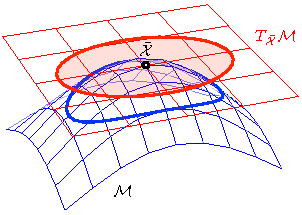
\includegraphics{figures/covariance}
\caption{围绕着点 $\bar\cX\in\cM$ 的不确定性被正确地表示为该点(红色)处向量空间的正切协方差。
使用 $\op$ 方程 \eqRef{equ:uncertainty},在切空间中的概率椭圆被缠绕在流形上(蓝色),从而说明了群上的概率集中区域。}
\label{fig:covariance}
\end{figure}




扰动也可以在全局参考中表示,即在原点 $\mtanat{\cM}{\cE}$ 处的切空间中,
使用左结合(left-)的 $\op$ 和 $\om$,
%
\begin{align}\label{equ:uncertainty_left}
\cX &= \bftau\op\bar\cX~, & \bftau &=\cX \om \bar\cX ~\in\mtanat{\cM}{\cE}
~.
\end{align}
%
这允许使用在方程 \eqRef{equ:cov} 中的左结合(left-)减号的协方差矩阵的全局规范。
例如,一个三维方向已知是在水平面中的旋转,可以与协方差矩阵 $^\cE\bfSigma=\diag(\sigma_\phi^2,\sigma_\theta^2, \infty)$ 相关联。
因为“水平(horizontal)”是一个全局规范,因此必须在全局参考中指定 $^\cE\bfSigma$ 。

%最后请注意,在这最后一点上没有达成共识。
%当文献 \cite{forster2017-TRO} 和我们使用局部扰动 $\cX=\bar\cX\op{^\cX\!\bftau}$ 时,文献 \cite{EADE-Lie,BARFOOT-14} 使用围绕原点的扰动, $\cX={^\cE\!\bftau}\op\bar\cX$,产生全局协方差规范。
因为全局扰动和局部扰动是由伴随方程 \eqRef{equ:Adj2} 联系起来的,它们的协方差的变换可以用
%
\begin{align}
^\cE\bfSigma_{\cX} = \Ad[\cM]{\cX} \, ^\cX\bfSigma_{\cX} \, \Ad[\cM]{\cX}\tr
~.
\end{align}

协方差的传播通过函数 $f:\cM\to\cN;\cX\mapsto \cY=f(\cX)$ 只需要用Jacobian矩阵方程 \eqRef{equ:Jacobian} 线性化方程 \eqRef{equ:lin_approx} 以获得熟悉的公式,
%
\begin{align}\label{equ:cov_propagation}
\bfSigma_{\cY} \approx \ndpar{f}{\cX} \, \bfSigma_\cX \, \ndpar{f}{\cX}\tr
~\in\bbR^{n\times n}
~.
\end{align}



%%%%%%%%%%%%%%%%%%%%%%%%%%%%%%%%%%%%%%%
\subsection{流形上的离散积分}

指数映射 $\cX(t)=\cX_0\circ\Exp(\bfv t)$ 执行恒定速度 $\bfv\in\mtanat{\cM}{\cX_0}$ 的连续时间积分到流形上。
非恒定速度 $\bfv(t)$ 通常通过将它们分割成分段恒定小量 $\bfv_k\in\mtanat{\cM}{\cX_{k-1}}$,(短的)持续时间为 $\dt_k$,并写成离散积分来处理
%
\begin{align*}
\cX_k &= \cX_0\circ\Exp(\bfv_1 \dt_1)\circ\Exp(\bfv_1 \dt_2)\circ\cdots\circ\Exp(\bfv_k \dt_k) \\
 &= \cX_0 \op \bfv_1 \dt_1\op\bfv_1 \dt_2\op\cdots\op\bfv_k \dt_k
~.
\end{align*}
%
等价地(\figRef{fig:manifold_int}),我们可以定义 $\bftau_k=\bfv_k\dt_k$ 并
将积分构造为(小的)离散正切步 $\bftau_k\in\mtanat{\cM}{\cX_{k-1}}$ 的 ``总和(sum)'',即,
%
$
\cX_k \te \cX_0\op\bftau_1\op\bftau_2\op\cdots\op\bftau_k.
$
%
我们用递归的形式写出所有这些变体,
%
\begin{align}\label{equ:int_recursive}
\cX_k = \cX_{k-1}\op\bftau_k = \cX_{k-1}\circ\Exp(\bftau_k) = \cX_{k-1}\circ\Exp(\bfv_k\dt_k)
~.
\end{align}
%

\begin{figure}[tb]
\centering
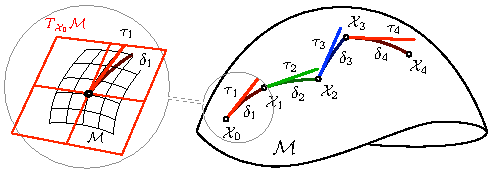
\includegraphics{figures/manifold_int}
\caption{流形上的运动积分。每一个运动数据生成一个步长 $\bftau_k\in\mtanat{\cM}{\cX_{k-1}}$,该步长被缠绕为局部运动增量或 `delta' $\delta_k=\Exp(\bftau_k)\in\cM$,然后与 $\cX_{k-1}$ 组合以产生 $\cX_k=\cX_{k-1}\circ\delta_k=\cX_{k-1}\circ\Exp(\bftau_k)=\cX_{k-1}\op\bftau_k\in\cM$.}
\label{fig:manifold_int}
\end{figure}%

常见的例子是将三维角速度 $\bfomega$ 积分到旋转矩阵, $\bfR_k=\bfR_{k-1}\Exp(\bfomega_k\dt)$,或积分到四元数 $\bfq_k=\bfq_{k-1}\Exp(\bfomega_k\dt)$。


% !TEX root = micro_Lie_theory.tex

%%%%%%%%%%%%%%%%%%%%%%%%%%%%%%%%%%%%%%%%%%%%%%%%%%%%%%%%%%%%
\section{流形上的微分法则}
\label{sec:derivatives_M}

对于我们所使用的所有经典流形 $\cM$ ,对于求逆(\emph{inversion})、组合(\emph{composition})、求幂(\emph{exponentiation})和作用(\emph{action})的初等Jacobian矩阵,我们可以确定封闭形式。
此外,其中一些形式可能与伴随 $\Ad[\cM]{\cX}$ 有关,后者成为微分过程的中心块。
$\Log$、 $\op$ 和 $\om$ 等其它形式可以很容易地从它们当中推导出来。
一旦找到这些形式或“块”,所有其它Jacobian矩阵都遵循链式法则。
除了我们下面介绍的所谓的左Jacobian矩阵(\emph{left Jacobian}),这里发展的所有Jacobian矩阵都是右Jacobian矩阵(\emph{right-Jacobian}),即由方程 \eqRef{equ:Jacobian} 所定义。
通过遵循这里的提示,感兴趣的读者应该不会发现在发展左Jacobian矩阵时有什么特别的困难。
对于不愿意这样做的读者,方程 \eqRef{equ:derivatives_lr_adjoints} 可用于此目的,因为


%
\begin{align}
\ldpar{f(\cX)}{\cX} = \Ad[\cN]{f(\cX)}\rdpar{f(\cX)}{\cX} \Ad[\cM]{\cX}\inv
~.
\end{align}


我们使用符号 $\mjac{f(\cX)}{\cX}\te\ndpar{f(\cX)}{\cX}$ 和 $\mjac{\cY}{\cX}\te\ndpar{\cY}{\cX}$ 。
我们还注意到, $\Ad[\cM]{\cX}\inv$ 应该由 $\Ad[\cM]{\cX\inv}$ 实现 ---参见方程 \eqssRef{equ:Adj5,equ:Adj7} 以及下面的注释。



\subsection{链式法则}
\label{sec:jacs_chain_rule}

对于 $\cY=f(\cX)$ 和 $\cZ=g(\cY)$ 我们有 $\cZ=g(f(\cX))$ 。
链式法则简单地说,
%
\begin{align}
\ndpar{\cZ}{\cX} = \ndpar{\cZ}{\cY}\,\ndpar{\cY}{\cX}
\qquad \textrm{or} \qquad
\mjac{\cZ}{\cX} = \mjac{\cZ}{\cY}\,\mjac{\cY}{\cX}
~.
\end{align}
%
我们为了右Jacobian矩阵在这里证明它,其中使用方程 \eqRef{equ:lin_approx} 三次,
%
\begin{align*}
g(f(\cX))\op\mjac{\cZ}{\cX}\bftau \gets g(f(\cX\op\bftau)) &\to g(f(\cX)~\op\mjac{\cY}{\cX}\bftau) 
  \\
  &\to g(f(\cX))\op\mjac{\cZ}{\cY}\mjac{\cY}{\cX}\bftau
\end{align*}
%
其中箭头表示极限为 $\bftau\to0$ ,因此 $\mjac{\cZ}{\cX}=\mjac{\cZ}{\cY}\mjac{\cY}{\cX}$ 。
左Jacobian矩阵和交叉Jacobian矩阵的证明类似,分别使用方程 \eqssRef{equ:lin_approx_left,equ:lin_approx_rl,equ:lin_approx_lr} 。
%
注意,当混合右、左和交叉Jacobian矩阵时,我们还需要链接参考帧,如
%
\begin{align}
\rldpar{\cZ}{\cX}
  &= \rrdpar{\cZ}{\cY}\,\rldpar{\cY}{\cX}
  = \rldpar{\cZ}{\cY}\,\lldpar{\cY}{\cX} \label{equ:chain_rule_cross_1}
\\
\lrdpar{\cZ}{\cX}
  &= \lrdpar{\cZ}{\cY}\,\rrdpar{\cY}{\cX}
  = \lldpar{\cZ}{\cY}\,\lrdpar{\cY}{\cX}\label{equ:chain_rule_cross_2}
~,
\end{align}
%
其中方程 \eqRef{equ:chain_rule_cross_1} 的第一个特征的证明通过写方程,
%
\begin{align*}
g(f({^\cE\!\bftau}\op\cX)) 
  &\xrightarrow[{^\cE\!\bftau}\to0]{\eqRef{equ:lin_approx_lr}} 
  g(f(\cX))\op\rldpar{\cZ}{\cX}\,{^\cE}\!\bftau
  ~; \\ 
g(f({^\cE\!\bftau}\op\cX)) 
  &\xrightarrow[{^\cE\!\bftau}\to0]{\eqRef{equ:lin_approx_lr}} 
  g\left(f(\cX)~\op\rldpar{\cY}{\cX}\,{^\cE}\!\bftau\right) \to
  \\
  &\xrightarrow[{^\cE\!\bftau}\to0]{\eqRef{equ:lin_approx}} 
  g(f(\cX))\op\rrdpar{\cZ}{\cY}\,\rldpar{\cY}{\cX}\,{^\cE}\!\bftau 
~,
\end{align*}
%
并在第一行和第三行中标识方程 \eqRef{equ:chain_rule_cross_1} 。


\subsection{初等Jacobian块}
\label{sec:jacs_elementary}

\subsubsection{求逆(Inverse)}
\label{sec:Jac_inversion}

我们用方程 \eqRef{equ:Jacobian} 定义 
%
\begin{align}
\mjac{\cX\inv}{\cX} 
  &\te \rdpar{\cX\inv}{\cX} \Quad\in \bbR^{m\times m}
  ~. \\
%
\intertext{这可以通过使用方程 \eqRef{equ:prop_exp} 和方程 \eqRef{equ:Adj4} 的伴随来确定,}
%
\mjac{\cX\inv}{\cX}\label{equ:Jac_inv}
  &= \lim_{\bftau\to0}\frac{\Log((\cX\inv)\inv(\cX\Exp(\bftau))\inv)}{\bftau} \notag\\
  &= \lim_{\bftau\to0}\frac{\Log(\cX\Exp(-\bftau)\cX\inv)}{\bftau} \notag \\
  &= \lim_{\bftau\to0}\frac{(\cX(-\bftau)^\wedge\cX\inv)^\vee}{\bftau} 
  = -\Ad[\cM]{\cX}
~.
\end{align}
%


\subsubsection{组合(Composition)}
\label{sec:Jac_composition}

我们用方程 \eqRef{equ:Jacobian} 定义
%
\begin{align}
\mjac{\cX\circ\cY}{\cX} &\te \rdpar{\cX\circ\cY}{\cX} &&\in \bbR^{m\times m} \\
\mjac{\cX\circ\cY}{\cY} &\te \rdpar{\cX\circ\cY}{\cY} &&\in \bbR^{m\times m}
~,
  \intertext{并如上面一样使用方程 \eqRef{equ:Adj4} 和方程 \eqRef{equ:Adj5},}
\mjac{\cX\circ\cY}{\cX} &= \Ad[\cM]{\cY}\inv \label{equ:Jac_comp_1}\\
\mjac{\cX\circ\cY}{\cY} &= \bfI \label{equ:Jac_comp_2}
\end{align}


\subsubsection[Right and left Jacobians]{Jacobians of $\cM$}

我们定义流形的右Jacobian矩阵(\emph{right Jacobian of $\cM$}) 为 $\cX=\Exp(\bftau)$ 的右Jacobian矩阵,即,对于 $\bftau\in
\bbR^m$ ,
%
\begin{align}
\mjac{}{r}(\bftau) \te \rdpar{\Exp(\bftau)}{\bftau} \in \bbR^{m\times m} 
~,
\label{equ:M_Jr}
\end{align}
%
这由方程 \eqRef{equ:Jacobian} 定义。 
右Jacobian矩阵将参数 $\bftau$ 的变化映射到 $\Exp(\bftau)$处的局部(\emph{local})切空间中的变化。
从方程 \eqRef{equ:Jacobian} 这很容易证明,对于小的 $\delta\bftau$ 值,以下近似值成立,
%
\begin{align}
\Exp(\bftau+\delta\bftau) &\approx \Exp(\bftau)\Exp(\mjac{}{r}(\bftau)\delta\bftau) \label{equ:Jr_1} \\
\Exp(\bftau)\Exp(\delta\bftau) &\approx \Exp(\bftau+\mjac{-1}{r}(\bftau)\,\delta\bftau) \label{equ:Jr_2} \\
\Log(\Exp(\bftau)\Exp(\delta\bftau)) &\approx \bftau+\mjac{-1}{r}(\bftau)\,\delta\bftau  \label{equ:Jr_3}
~.
\end{align}
%

作为补充,流形的左Jacobian矩阵(\emph{left Jacobian of $\cM$})被定义为, 
%
\begin{align}
\mjac{}{l}(\bftau) \te \ldpar{\Exp(\bftau)}{\bftau} \in \bbR^{m\times m} 
~,
\label{equ:M_Jl}
\end{align}
%
使用左Jacobian矩阵方程 \eqRef{equ:left-Jacobian},得出近似值
%
\begin{align}
\Exp(\bftau+\delta\bftau) &\approx \Exp(\mjac{}{l}(\bftau)\delta\bftau)\Exp(\bftau)  \label{equ:Jl_1}\\
\Exp(\delta\bftau)\Exp(\bftau) &\approx \Exp(\bftau+\mjac{-1}{l}(\bftau)\,\delta\bftau)  \label{equ:Jl_2}\\
\Log(\Exp(\delta\bftau)\Exp(\bftau)) &\approx \bftau+\mjac{-1}{l}(\bftau)\,\delta\bftau  \label{equ:Jl_3}
~.
\end{align}
% 
左Jacobian矩阵将参数 $\bftau$ 的变化映射到全局(\emph{global})切空间或Lie代数中的变化。
从方程 ~\eqssRef{equ:Jr_1,equ:Jl_1} 我们可以把左Jacobian矩阵和右Jacobian矩阵用伴随联系起来,
%
\begin{align}\label{equ:Jr_Jl_Adj}
\Ad[\cM]{\Exp(\bftau)} = \mjac{}{l}(\bftau)\,\mjac{}{r}\inv(\bftau)
~.
\end{align}
%
此外,链式法则允许我们关联 $\mjac{}{r}$ 和 $\mjac{}{l}$,
%
\begin{align}\label{equ:Jr_minus}
\mjac{}{r}(-\bftau) 
  &\te \mjac{\Exp(-\bftau)}{-\bftau} 
  = \mjac{\Exp(-\bftau)}{\bftau}\mjac{\bftau}{-\bftau} 
  = \mjac{\Exp(\bftau)\inv}{\bftau}(-\bfI) 
  \notag\\
  &
  = -\mjac{\Exp(\bftau)\inv}{\Exp(\bftau)}\mjac{\Exp(\bftau)}{\bftau} 
  = \Ad{\Exp(\bftau)}\mjac{}{r}(\bftau)
  \notag\\
  &
  = \mjac{}{l}(\bftau)
  ~.
\end{align}



对于使用中的经典流形, $\mjac{}{r}$、 $\mjac{}{r}\inv$、 $\mjac{}{l}$ 和 $\mjac{}{l}\inv$ ,存在封闭形式。
查询请参考附件。


\subsubsection{群作用}


对于 $\cX\in\cM$ 和 $v\in\cV$我们用方程 \eqRef{equ:Jacobian} 定义
%
\begin{align}
\mjac{\cX\cdot v}{\cX} &\te \rdpar{\cX\cdot v}{\cX} \\
\mjac{\cX\cdot v}{v}   &\te \rdpar{\cX\cdot v}{v} 
~.
\end{align}
%
由于群作用依赖于集合 $\cV$,因此这些表达式不能通用化。
查询请参考附件。



\subsection{有用的,但可推导的, Jacobian 矩阵块}

\subsubsection[Log map]{$\Log$ 映射}

对于 $\bftau=\Log(\cX)$ ,
并从方程 \eqRef{equ:Jr_3} ,
%
\begin{align}\label{equ:Jac_log}
\mjac{\Log(\cX)}{\cX} 
&= \mjac{-1}{r}(\bftau) 
~.
\end{align}

\subsubsection{加号和减号}

我们有
%
\begin{align}
\mjac{\cX\op\bftau}{\cX}
  &= \mjac{\cX\circ(\Exp(\bftau))}{\cX} 
  ~~~~~~~~~= \Ad[\cM]{\Exp(\bftau)}\inv \\
\mjac{\cX\op\bftau}{\bftau}
  &= \mjac{\cX\circ(\Exp(\bftau))}{\Exp(\bftau)}\mjac{\Exp(\bftau)}{\bftau}
  = \mjac{}{r}(\bftau) 
\end{align}
%
并得到 $\cZ=\cX\inv\circ\cY$ 和 $\bftau=\cY\om\cX=\Log(\cZ)$ ,
%
\begin{align}
\mjac{\cY\om\cX}{\cX}
  &= \mjac{\Log(\cZ)}{\cZ}\mjac{\cZ}{\cX\inv}\mjac{\cX\inv}{\cX} 
   = -\mjac{-1}{l}(\bftau)
  \\
\mjac{\cY\om\cX}{\cY}
  &= \mjac{\Log(\cZ)}{\cZ}\mjac{\cZ}{\cY} 
  ~~~~~~~~~= \mjac{-1}{r}(\bftau)
~.
\end{align}
%
在这里证明前者
%
\begin{align*}
\mjac{\cY\om\cX}{\cX}
  &= \mjac{\Log(\cX\inv\circ\cY)}{(\cX\inv\circ\cY)}\,\mjac{(\cX\inv\circ\cY)}{\cX\inv}\,\mjac{\cX\inv}{\cX} 
 \notag\\ 
 (\ref{equ:Jac_log},\ref{equ:Jac_comp_1},\ref{equ:Jac_inv})
  &= ~~\,\mjac{-1}{r}(\bftau)~~\Ad[\cM]{\cY}\inv~~(-\Ad[\cM]{\cX}) 
 \notag\\ 
 (\ref{equ:Adj5},\ref{equ:Adj7})
  &= -\mjac{-1}{r}(\bftau)\,\Ad[\cM]{\cY\inv\cX} 
 \notag\\ 
  &= -\mjac{-1}{r}(\bftau)\,\Ad[\cM]{\Exp(\bftau)}\inv
  \notag\\
 (\ref{equ:Jr_Jl_Adj})
  &
  =  -\mjac{-1}{l}(\bftau)
  ~.
\end{align*}






% Extras
% !TEX root = micro_Lie_theory.tex


\section{组合流形}

以失去与Lie理论的某些一致性为代价,但以获得符号和操作方面的一些优势为好处,人们可以将大的和非均匀的状态视为流形组合(或捆绑)。


\if \examples y % !TEX root = micro_Lie_theory.tex

%%%%%%%%%%%%%%%%%%%%%%%% Composite %%%%%%%%%%%%%%%%%%%%%%%
\begin{fexample}{$\SE(n)$ \emph{vs.} $T(n) \tcross \SO(n)$ \emph{vs.} 
$\langle\bbR^n,\SO(n)\rangle$}
%the composite}
\label{ex:sen_sonxrn_comp}

我们考虑平移空间 $\bft\in\bbR^n$ 和旋转空间 $\bfR\in\SO(n)$。
为此,我们有著名的 $\SE(n)$ 刚体运动流形 $\bfM=\begin{bsmallmatrix}\bfR&\bft\\\bf0&1\end{bsmallmatrix}$ (参见 Apps.~\ref{sec:SE2} 和 \ref{sec:SE3}),这也可以构造为 $T(n) \tcross \SO(n)$ (参见 Apps.~\ref{sec:S1_SO2}, \ref{sec:S3_SO3} 和 \ref{sec:Tn})。
这两者非常相似,但有不同的正切参数化:
当 $\SE(n)$ 使用 $\bftau=(\bth,\bfrho)$ 和 $\bfM=\exp(\bftau^\wedge)$ , 
而 $T(n) \tcross \SO(n)$ 使用 $\bftau=(\bth,\bfp)$ 和 $\bfM=\exp(\bfp^\wedge)\exp(\bth^\wedge)$ 。
它们共享旋转部分 $\bth$,但显然是 $\bfrho\ne\bfp$ (对于更多详细信息,参见文献 \cite[pag.~35]{CHIRIKJIAN-11})。
简而言之,$\SE(n)$ 作为一个连续体同时执行平移和旋转,
而 $T(n) \tcross \SO(n)$ 执行链式平移+旋转。
相反,在组合 $\langle\bbR^n,\SO(n)\rangle$ 中,旋转和平移根本不相互作用。
通过用 $\Exp()$ 将组合结合,我们得到(右)加号算子,
%
\begin{align*}
\SE(n)&:& 
\bfM\oplus\bftau &= \begin{bmatrix}
\bfR\Exp(\bth) & \bft+\bfR\bfV(\bth)\bfrho \\
\bf0 & 1
\end{bmatrix} 
\\
T(n) \tcross \SO(n)&:&
\bfM\oplus\bftau &= \begin{bmatrix}
\bfR\Exp(\bth) & \bft+\bfR\bfp \\
\bf0 & 1
\end{bmatrix} 
\\ 
\langle\bbR^n,\SO(n)\rangle&:&
\bfM\dplus\bftau 
& 
= 
\begin{bmatrix}
\bft+\bfp \\
\bfR\Exp(\bth)
\end{bmatrix} 
\end{align*}
%
其中 $\oplus$ 可用于系统动力学,例如运动积分,但通常不用 $\dplus$,后者可用于对扰动进行建模。
%
它们各自的减号算子读取,
%. 
\begin{align*}
\SE(n)&:&
\bfM_2\ominus\bfM_1 & = \begin{bmatrix}
\bfV_1\inv\bfR_1\tr(\bfp_2 - \bfp_1) \\ \Log(\bfR_1\tr\bfR_2)
\end{bmatrix} 
\\
T(n) \tcross \SO(n)&:&
\bfM_2\ominus\bfM_1 & = \begin{bmatrix}
\bfR_1\tr(\bfp_2 - \bfp_1) \\ \Log(\bfR_1\tr\bfR_2)
\end{bmatrix} 
\\
\langle\bbR^n,\SO(n)\rangle&:&
\bfM_2\dminus\bfM_1 
&= 
\begin{bmatrix}
\bfp_2 - \bfp_1 \\ \Log(\bfR_1\tr\bfR_2)
\end{bmatrix} 
~,
\end{align*}
%
现在这里有趣的是, $\dminus$ 可以用来评估误差和不确定性。这使得 $\dplus,\dminus$ 成为计算导数和协方差的有价值的算子。
\end{fexample}
%%%%%%%%%%%%%%%%%%%%%%%%%%%%%%%%%%%%%%%%%%%%%%%%%%
 \fi


一个组合流形(\emph{composite manifold}) $\cM=\langle\cM_1,\cdots,\cM_M\rangle$ 不小于 $M$ 个非相互作用的流形的级联。
这源于幺元、逆元的定义,以及单独地在每一个块上的组合作用的组合,
%
\begin{align}
\cE_\diamond &\te \begin{bmatrix}
\cE_1 \\ \vdots \\ \cE_M
\end{bmatrix},
&
\cX^\diamond &\te \begin{bmatrix}
\cX\inv \\ \vdots \\ \cX_M\inv
\end{bmatrix},
&
\cX\diamond\cY &\te \begin{bmatrix}
\cX\circ\cY_1 \\
\vdots\\
\cX_M\circ\cY_M 
\end{bmatrix}
,
\end{align}
%
从而实现了群公理,以及一个非相互作用的收回映射,为了统一符号(注意尖括号),我们还将其标记为“指数映射”,
%
\begin{align}\label{equ:exp_composite}
\Exp\langle\bftau\rangle &\te \begin{bmatrix}
\Exp(\bftau_1) \\ \vdots \\ \Exp(\bftau_M)
\end{bmatrix}
\,,
&
\Log\langle\cX\rangle &\te \begin{bmatrix}
\Log(\cX) \\ \vdots \\ \Log(\cX_M)
\end{bmatrix}
,
\end{align}
% 
从而确保平滑。
这些产生了组合的右结合(right-)的加号和减号(注意菱形符号),
%
\begin{align}
\cX\dplus\bftau &\te \cX\diamond\Exp\langle\bftau\rangle \\
\cY\dminus\cX &\te \Log\langle\cX^\diamond\diamond\cY\rangle
~.
\end{align}

这些考虑的关键结果%
\if\examples y{ (参见 Ex.~\ref{ex:sen_sonxrn_comp}) }\else { }\fi 
是可以定义新的导数,\footnotemark\ 使用 $\dplus$ 和 $\dminus$ ,
\footnotetext{这里我们假设右导数,但同样适用于左导数。}
%
\begin{align}
\ndpar{f(\cX)}{\cX} \te \lim_{\bftau\to0}\frac{f(\cX\dplus\bftau)\dminus f(\cX)}{\bftau}
\label{equ:Jacobian_composite}
~.
\end{align}
%
利用这个导数,作用在组合流形上的函数 $f:\cM\to\cN$ 的Jacobian矩阵可以按块计算来确定,这就产生了只需要知道组合的流形块的简单表达式,
%
\begin{align}
\ndpar{f(\cX)}{\cX} &= \begin{bmatrix}
\ndpar{f_1}{\cX_1} & \cdots & \ndpar{f_1}{\cX_M} \\
\vdots             & \ddots & \vdots \\
\ndpar{f_N}{\cX_1} & \cdots & \ndpar{f_N}{\cX_M} \\
\end{bmatrix}
~,
\end{align}
%
其中, $\ndpar{f_i}{\cX_j}$ 分别用方程 \eqRef{equ:Jacobian} 计算。 
对于 $\bftau$ 的小值,以下方程成立,
%
\begin{align}\label{equ:lin_approx_composite}
f(\cX\dplus\bftau) \xrightarrow[{\bftau}\to0]{} f(\cX)\dplus\ndpar{f(\cX)}{\cX}\,{\bftau}
\quad \in \cN
~.
\end{align}

当使用这些导数时,协方差和不确定性传播必须遵循约定。特别是,协方差矩阵方程 \eqRef{equ:cov} 变成
%
\begin{align}\label{equ:cov_composite}
\bfSigma_\cX \te \bbE[(\cX \dminus \bar\cX)(\cX \dminus \bar\cX)\tr]~\in\bbR^{n\times n}
~,
\end{align}
%
对于线性化传播方程 \eqRef{equ:cov_propagation} ,使用方程 \eqRef{equ:Jacobian_composite} 以应用它。



% Examples
%\input{homogeneous.tex}
% !TEX root = micro_Lie_theory.tex

\newcommand{\dx}{{\delta\bfx}}

\section{基于地标的定位与建图}
\label{sec:SLAM}

我们提供了三个机器人定位和建图理论的应用实例。 
第一个是基于Kalman滤波的地标定位方法。
第二个是基于图的平滑方法,用于同时定位和建图。
第三个增加了传感器自校正。
它们基于一个公共设置,解释如下。

我们考虑一个在平面上的机器人
(对于三维情况,参见 \secRef{sec:demos_3D})
周围有少量准时的地标或信标(\emph{beacons})。 
机器人以轴向速度和角速度的形式接收控制动作,并且能够测量信标相对于其自身参考坐标系的位置。


机器人姿态在 $\SE(2)$ 中 (\appRef{sec:SE2}) ,并且信标位置在 $\bbR^2$ 中 (\appRef{sec:Tn}),
%
\begin{align*}
\cX &= 
\begin{bmatrix}
\bfR & \bft \\ \bf0 & 1
\end{bmatrix}\in\SE(2)
~,
&
\bfb_k &= \begin{bmatrix}
x_k \\ y_k
\end{bmatrix}\in\bbR^2
~.
\end{align*}

控制信号 $\bfu$ 是 $\se(2)$ 中的一个扭曲,包括纵向速度 $v$ 和角速度 $\omega$,没有横向速度分量,在采样时间 $\dt$ 内积分。
该控制已被加性高斯噪声 $\bfw\sim\cN(\bf0,\bfW)$ 损坏。
此噪声可能视为车轮横向打滑 $u_s$ ,数值为 $\sigma_s\ne0$,
%
\begin{align}
\bfu &
= \begin{bmatrix} u_v \\ u_s \\ u_\omega \end{bmatrix} 
= \begin{bmatrix} v\,\dt \\ 0 \\ \omega\,\dt \end{bmatrix}+\bfw  
&&\in\se(2)
\\
\bfW &= \begin{bmatrix}
\sigma_v^2\dt &0&0 \\ 0&\sigma_s^2\dt&0 \\ 0&0&\sigma_w^2\dt
\end{bmatrix} &&\in\bbR^{3\times3}.
\end{align}
%
当一个控制 $\bfu_j$ 在时间 $j$ 到达时,机器人的姿态将更新为方程 \eqRef{equ:int_recursive},
%
\begin{align}\label{equ:motion}
\cX_j &= \cX_i \op \bfu_j \te \cX_i \Exp(\bfu_j)
~.
\end{align}


%
地标测量是有范围和承载类型的,尽管为了简单起见,它们被放在笛卡尔形式中。
它们的噪声 $\bfn\sim\cN({\bf0},\bfN)$ 是零均值高斯分布,
%
\begin{align}\label{equ:meas_beacon}
\bfy_k &= \cX\inv\cdot\bfb_k + \bfn = \bfR\tr(\bfb_k-\bft) + \bfn	&&\in \bbR^2
\\
\bfN &= \begin{bmatrix}
\sigma_x^2 &0 \\ 0& \sigma_y^2
\end{bmatrix}										&&\in\bbR^{2\times2}
~,
\end{align}
%
其中我们注意到刚体运动作用 $\cX\inv\cdot\bfb_k$ (参见 \appRef{sec:SE2})。




%%%%%%%%%%%%%%%%%%%%%%%%%%%%%%%%%%%%%%%%%%%%%%%%%%%%%%%%%%%%%%%%
\subsection{基于流形的误差状态Kalman滤波定位}
\label{sec:loc_ESKF}

我们最初考虑信标 $\bfb_k$ 位于已知位置。 
我们将要估计的姿态定义为 $\hat\cX\in\SE(2)$。
估计误差 $\dx$ 及其协方差 $\bfP$ 在 $\hat\cX$ 处切空间中用方程 \eqssRef{equ:uncertainty,equ:cov} 表示,
%
\begin{align}\label{equ:loc_Gaussian}
\dx &\te \cX\ominus\hat\cX && \in\bbR^3
\\
\bfP &\te \bbE[(\cX\ominus\hat\cX)(\cX\ominus\hat\cX)\tr]&& \in\bbR^{3\times3}
~.
\end{align}
%
在机器人的每一个运动中,我们应用ESKF预测,
%
\begin{align}
\hat\cX_j &= \hat\cX_i\op\bfu_j \label{equ:loc_ekf_pred}
\\
\bfP_j &= \bfF\,\bfP_i\,\bfF\tr + \bfG\,\bfW_j\,\bfG\tr
~,
\end{align}
%
用 \appRef{sec:SE2} 中的块计算 Jacobians 矩阵,
%
\begin{align*}
\bfF &\te \mjac{\cX_j}{\cX_i} = \mjac{\hat\cX_i\op\bfu_j}{\hat\cX_i} 
= \Ad{\Exp(\bfu_j)}\inv
\\
\bfG &\te \mjac{\cX_j}{\bfu_j} = \mjac{\hat\cX_i\op\bfu_j}{\bfu_j} = \mjac{}{r}(\bfu_j)
~.
\end{align*}
%
在每个信标测量 $\bfy_k$ 时,我们应用ESKF校正,
%
\begin{align}
\textrm{Innovation}&:&\bfz &= \bfy_k - \hat\cX\inv\cdot\bfb_k \notag\\
\textrm{Innovation cov.}&:&\bfZ &= \bfH\,\bfP\,\bfH\tr+\bfN \notag\\
\textrm{Kalman gain}&:&\bfK &= \bfP\,\bfH\tr\,\bfZ\inv \notag\\
\textrm{Observed error}&:&\dx &= \bfK\bfz \notag\\
\textrm{State update}&:&\hat\cX &\gets \hat\cX \oplus \dx \label{equ:loc_ekf_corr}\\
\textrm{Cov. update}&:&\bfP &\gets \bfP - \bfK\,\bfZ\,\bfK\tr
~,
\end{align}
%
用 \appRef{sec:SE2} 中的块计算 Jacobians 矩阵,
\begin{align*}
\bfH 
&\te \mjac{\cX\inv\cdot\bfb_k}{\cX}= \mjac{\cX\inv\cdot\bfb_k}{\cX\inv}\,\mjac{\cX\inv}{\cX} 
\notag\\
&= 
\begin{bmatrix}\bfR\tr & \bfR\tr\hatx{1}\bfb_k\end{bmatrix}
\begin{bmatrix}
-\bfR & \hatx{1}\bft \\ \bf0 & -1
\end{bmatrix}
\notag\\
&=
-\begin{bmatrix}\bfI & \bfR\tr\hatx{1}(\bfb_k-\bft)\end{bmatrix}
~.
\end{align*}

注意,相对于常规EKF的唯一更改在方程 \eqRef{equ:loc_ekf_pred} 和方程 \eqRef{equ:loc_ekf_corr},其中常规的 $+$ 被用 $\op$ 替换。
相反地,Jacobian矩阵都用Lie理论计算(参见 \appRef{sec:SE2})。
有趣的是,它们的用法与标准EKF中的用法相同 --- 例如,参见Kalman增益方程,即标准的 $\bfK = \bfP\bfH\tr(\bfH\bfP\bfH\tr+\bfN)\inv$ 。


%%%%%%%%%%%%%%%%%%%%%%%%%%%%%%%%%%%%%%%%%%%%%%%%%%%%%%%%%%%%%%%%
\subsection{基于图优化的平滑和建图}
\label{sec:SAM}

我们现在考虑平滑和映射(SAM)问题,其中要估计的变量是信标的位置和机器人的轨迹。
选择的解算器是一个基于图的迭代最小二乘优化器。
为简单起见,我们假设轨迹由三个机器人姿态 $\{\cX_1\cdots\cX_3\}$ ,一个有三个信标 $\{\bfb_4\cdots\bfb_6\}$ 的世界组成。
问题状态是组合的
%
\begin{align}\label{equ:SAM_state}
\cX &= \langle
\cX_1 , \cX_2 , \cX_3 , \bfb_4 , \bfb_5 , \bfb_6
\rangle, \quad \cX_i\in\SE(2),\quad\bfb_k\in\bbR^2.
\end{align}
%
结果因子图 \cite{DELLAERT-IJRR-06} 如 \figRef{fig:graph-SLAM} 所示。
每一个先验或测量值在图中贡献一个因子。
从姿态 $i$ 到 $j$ 的运动测量值来自方程 \eqRef{equ:motion},
当信标 $k$ 从姿态 $i$ 的测量时响应方程 \eqRef{equ:meas_beacon},
%
\begin{figure}
\centering
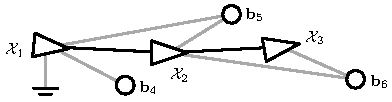
\includegraphics{figures/SAM}
\caption{具有3个姿态和3个信标的SAM因子图。
每一个测量值在图中贡献一个因子。
这里有2个运动因子(黑色)和5个信标因子(灰色)。
在 $\cX_1$ 上的先验因子提供全局可观测性。}
\label{fig:graph-SLAM}
\end{figure}
%
%
\begin{align}
\bfu_{ij} &= \cX_j\ominus\cX_i + \bfw_{ij} = \Log(\cX_i\inv\cX_j) + \bfw_{ij} \label{equ:meas_motion} \\
\bfy_{ik} &= \cX_i\inv\cdot\bfb_k + \bfn_{ik}
~.
\end{align}
%
每一个因子都有一个信息矩阵, $\bfOmega_{1} \te \bfW_{1}\inv$, $\bfOmega_{ij} \te \bfW_{ij}\inv$ 和 $\bfOmega_{ik} \te \bfN_{ik}\inv$ 。
%
期望残差(residual)是,
%
\begin{align}
\textrm{prior residual}&:&\bfr_{1}(\cX) &= \bfOmega_{1}^{\top/2}(\cX_1 \om \hat\cX_1)
\notag
\\
\textrm{motion residual}&:&\bfr_{ij}(\cX) &= \bfOmega_{ij}^{\top/2}(\bfu_{ij} - (\hat\cX_j\ominus\hat\cX_i))
\notag
\\
\textrm{beacon residual}&:&\bfr_{ik}(\cX) &= \bfOmega_{ik}^{\top/2}(\bfy_{ik} - \hat\cX_i\inv\cdot\hat\bfb_k)
\notag
~.
\end{align}
%
最佳更新步骤 $\dx$ 源自于最小化
%
\begin{align}\label{equ:SAM_problem}
\dx^* = \argmin_{\dx} \sum_{p\in\cP} \bfr_p(\cX\dplus\dx)\tr\bfr_p(\cX\dplus\dx)
\end{align}
%
其中 $\cP=\{1,12,23,14,15,25,26,36\}$ 是每一个测量的节点对的集合 (参见 \figRef{fig:graph-SLAM}) 。
这个问题迭代求解如下。
总和方程 \eqRef{equ:SAM_problem} 中的每一个残差跟随方程 \eqRef{equ:lin_approx_composite} 被线性化为 $\bfr_p(\cX\dplus\dx)\approx\bfr_p(\cX)\dplus\mjac{\bfr_p}{\cX}\dx$ ,其中 $\mjac{\bfr_p}{\cX}$ 是稀疏Jacobian矩阵。
这些Jacobian矩阵的非零块,即 $\mjac{\bfr_{1}}{\cX_1}$, $\mjac{\bfr_{ij}}{\cX_i}$, $\mjac{\bfr_{ij}}{\cX_j}$, $\mjac{\bfr_{ik}}{\cX_i}$ 和 $\mjac{\bfr_{ik}}{\bfb_k}$,可以按照 \secRef{sec:loc_ESKF} 中的方法轻松计算,并注意到根据定义 $\mjac{f(\cX\op\dx)}{\dx}|_{\dx=0}=\mjac{f(\cX\op\dx)}{\cX}|_{\dx=0}=\mjac{f(\cX)}{\cX}$。
%
建立总的Jacobian矩阵和残差向量,
%
\begin{align}\label{equ:SAM_problem_lin}
\bfJ &= \begin{bmatrix}
\mjac{\bfr_{1}}{\cX_1} & \bf0 & \bf0 & \bf0 & \bf0 & \bf0 \\ 
\mjac{\bfr_{12}}{\cX_1} & \mjac{\bfr_{12}}{\cX_2} & \bf0 & \bf0 & \bf0 & \bf0 \\ 
\bf0 & \mjac{\bfr_{23}}{\cX_2} & \mjac{\bfr_{23}}{\cX_3} & \bf0 & \bf0 & \bf0 \\ 
\mjac{\bfr_{14}}{\cX_1} & \bf0 & \bf0 & \mjac{\bfr_{14}}{\bfb_4} & \bf0 & \bf0 \\ 
\mjac{\bfr_{15}}{\cX_1} & \bf0 & \bf0 & \bf0 & \mjac{\bfr_{15}}{\bfb_5} & \bf0 \\ 
\bf0 & \mjac{\bfr_{25}}{\cX_2} & \bf0 & \bf0 & \mjac{\bfr_{25}}{\bfb_5} & \bf0 \\ 
\bf0 & \mjac{\bfr_{26}}{\cX_2} & \bf0 & \bf0 & \bf0 & \mjac{\bfr_{26}}{\bfb_6} \\ 
\bf0 & \bf0 & \mjac{\bfr_{36}}{\cX_3} & \bf0 & \bf0 & \mjac{\bfr_{36}}{\bfb_6} 
\end{bmatrix}
&
\bfr &= \begin{bmatrix}
\bfr_{1} \\
\bfr_{12} \\
\bfr_{23} \\
\bfr_{14} \\
\bfr_{15} \\
\bfr_{25} \\
\bfr_{26} \\
\bfr_{36}
\end{bmatrix}
\end{align}
%
线性化的方程 \eqRef{equ:SAM_problem} 现在转换为 \cite{DELLAERT-IJRR-06} 最小化
%
\begin{align}
\dx^* 
 &= \argmin_\dx \norm{\bfr+\bfJ\dx}^2
.
\end{align}
%
这通过使用 $\bfJ$ 的伪逆的最小二乘法来解决 (对于大型问题,需要 QR \cite{DELLAERT-IJRR-06,KAESS-11-ISAM2} 或 Cholesky \cite{KUMMERLE-11-G2O,ILA-17_SLAM++} 的因式分解),
%
\begin{align}
\dx^* &= -(\bfJ\tr\bfJ)\inv\bfJ\tr\bfr \label{equ:SAM_opt_step}
~,
\intertext{产生用于更新状态的最佳步骤 $\dx^*$ ,}
\cX &\gets \cX \dplus \dx^* \label{equ:SAM_update}
~.
\end{align}
%
这个过程被迭代直到收敛。

我们在此强调在方程 \eqRef{equ:SAM_state} 中组合符号的使用,它允许按块定义Jacobian矩阵方程 \eqRef{equ:SAM_problem_lin} 和更新方程 \eqRef{equ:SAM_update} 。我们还注意到 $\SE(2)$ 流形在运动和测量模型中的使用,正如我们在 \secRef{sec:loc_ESKF} 中的ESKF案例中所做的那样。


%%%%%%%%%%%%%%%%%%%%%%%%%%%%%%%%%%%%%%%%%%%%%%%%%%%%%%%%%%%%%%%%
\subsection{自校正平滑和建图}

我们考虑与上述问题相同的问题,但运动传感器受到未知校正偏差 $\bfc=(c_v,c_\omega)\tr$ 的影响,
 所以控制现在是 $
\tilde\bfu 
=
(v\dt + c_v ,~
0 ,~
\omega \dt + c_\omega)\tr + \bfw
$.
%
我们定义偏差校正函数 $c()$ ,
%
\begin{align}\label{equ:bias}
\bfu &= c\,(\tilde\bfu, \bfc) \te \begin{bmatrix}
\tilde u_v - c_v \\
\tilde u_s \\
\tilde u_\omega - c_\omega
\end{bmatrix} \quad \in \bbR^3\cong\se(2)
~.
\end{align}
%
状态组合用未知的 $\bfc$ 扩充,
%
\begin{align*}
\cX &= \langle
\bfc, \cX_1 , \cX_2 , \cX_3 , \bfb_4 , \bfb_5 , \bfb_6
\rangle
~, 
\\
\bfc&\in\bbR^2,\qquad\cX_i\in\SE(2),\qquad\bfb_k\in\bbR^2
~,
\end{align*}
%
并且运动残差变为
%
\begin{align*}
\bfr_{ij}(\cX) &= \bfOmega_{ij}^{\top/2}\big(c\,(\tilde\bfu_{ij} , \bfc) - (\hat\cX_j\ominus\hat\cX_i)\big)
~.
\end{align*}
%
步骤如上面 \secRef{sec:SAM} 一样,并且总Jacobian矩阵在左边加了一列,
%
\begin{align*}
\bfJ &= \begin{bmatrix}
\bf0 & \mjac{\bfr_{1}}{\cX_1} & \bf0 & \bf0 & \bf0 & \bf0 & \bf0 \\ 
\mjac{\bfr_{12}}{\bfc} & \mjac{\bfr_{12}}{\cX_1} & \mjac{\bfr_{12}}{\cX_2} & \bf0 & \bf0 & \bf0 & \bf0 \\ 
\mjac{\bfr_{23}}{\bfc} & \bf0 & \mjac{\bfr_{23}}{\cX_2} & \mjac{\bfr_{23}}{\cX_3} & \bf0 & \bf0 & \bf0 \\ 
\bf0 & \mjac{\bfr_{14}}{\cX_1} & \bf0 & \bf0 & \mjac{\bfr_{14}}{\bfb_4} & \bf0 & \bf0 \\ 
\bf0 & \mjac{\bfr_{15}}{\cX_1} & \bf0 & \bf0 & \bf0 & \mjac{\bfr_{15}}{\bfb_5} & \bf0 \\ 
\bf0 & \bf0 & \mjac{\bfr_{25}}{\cX_2} & \bf0 & \bf0 & \mjac{\bfr_{25}}{\bfb_5} & \bf0 \\ 
\bf0 & \bf0 & \mjac{\bfr_{26}}{\cX_2} & \bf0 & \bf0 & \bf0 & \mjac{\bfr_{26}}{\bfb_6} \\ 
\bf0 & \bf0 & \bf0 & \mjac{\bfr_{36}}{\cX_3} & \bf0 & \bf0 & \mjac{\bfr_{36}}{\bfb_6} 
\end{bmatrix}
~,
\end{align*}
%
其中 $\mjac{\bfr_{ij}}{\bfc} = \bfOmega_{ij}^{\top/2}\mjac{c(\bfu_{ij} , \bfc)}{\bfc}$,其中 $\mjac{c(\bfu_{ij} , \bfc)}{\bfc}$ 是方程 \eqRef{equ:bias} 的 $3\times 2$ 的Jacobian矩阵。
最优解用方程 \eqssRef{equ:SAM_opt_step,equ:SAM_update} 获得。
得到的最优状态 $\cX$ 包括 $\bfc$ 的最优估计,即传感器偏差的自校正。

\subsection{3D实现}
\label{sec:demos_3D}

把上面所有的例子都放到3D上是非常容易的。
在正确的空间中定义所有变量就足够了:
$\cX\in\SE(3)$ 和 $\bfu\in\bbR^6\cong\se(3)$ (\appRef{sec:SE3}), 和 $\{\bfb_k,\bfy\}\in\bbR^3$ (\appRef{sec:Tn})。
Jacobian矩阵和协方差矩阵将遵循适当的大小。
%
这里有趣的地方在于认识到算法中的所有数学,即从方程 \eqRef{equ:loc_Gaussian} 出发,对于2D和3D来说是完全一样的:Lie理论提供的抽象层次使这成为可能。



% Applications
%\input{self_calib.tex}
%\input{imu_preintegration.tex}
%\input{imu.tex}
%% !TEX root = micro_Lie_theory.tex

\section{差动驱动自校正}
\label{sec:diff_drive}

%%%%%%%%%%%%%%%%%%%%%%%%%%%%%%%%%%%%%%%%%%%%%%%%%%%%%%%%%%%%
\subsection{概述}

差动驱动模型由两种驱动轮组成,一种在单轴上,一种位于机器人基座的每一侧,
其原点坐标系位于轴线的中心。
机器人的参数化由
它的轮子的半径 $(r_l, r_r)$ 和轴线的长度 $d$ 确定。
与每一个参数中的相关联的是一个校正因子,使得
$\bfc=[c_l~c_r~c_d]\tr$ 是内在参数校正向量。
%
通常通过车轮编码器测量运动,报告车轮增量角度 $\bfy=[\delta\psi_l, \delta\psi_r]+\bfn$ ,
在每个时间步长 $\delta t$ 处,其中 $\bfn$ 是加性高斯噪声。


%%%%%%%%%%%%%%%%%%%%%%%%%%%%%%%%%%%%%%%%%%%%%%%%%%%%%%%%%%%%
\subsection{State and delta definitions}
%
We define the states of position and orientation angle
$\bfx = (\bfp,\theta)$, which act as a compact representation of $SE(2)$.
Consequently, state increments or deltas $\D_{ij}$ and $\delta_k$ are also in $SE(2)$.


%
%%%%%%%%%%%%%%%%%%%%%%%%%%%%%%%%%%%%%%%%%%%%%%%%%%%%%%%%%%%%
\subsection{Delta pre-integration}

For convenience, we define the body magnitudes 
$\bfb = (\delta l,\delta \theta)=f_b(\bfy,\bfc,\bfn)$ as
%
%
\begin{align}
\label{equ:diff_drive_psis}
\begin{split}
\delta l &= \tfrac12(r_r c_r \delta\psi_r + r_l c_l\delta\psi_l)  \\
\delta \theta &= \tfrac{1}{D}(r_r c_r \delta\psi_r - r_l c_l\delta\psi_l) 
~.
\end{split}
\end{align}
%
with $D=d\,c_d$. 
Its components, respectively, highlight the common (along track length), and differential (turn) components of the wheels reported motions.

Assuming constant control inputs over the sampling time period $[t_j,t_k]$, the robot
moves along an arc of circle of radius
%
\begin{align}
R = \frac{\delta l}{\delta \theta} 
~.
\end{align}
%
The motion increment $\delta_k$ can be expressed in $SE(2)$ as
%
\begin{align}
\label{equ:diff_drive_exact_inte}
\delta x &= R\sin(\delta\theta) \notag\\
\delta y &= R(1-\cos(\delta\theta)) \\
\delta\theta &= \delta \theta \notag 
~,
\end{align}
%
which is exactly $\delta=\Exp(\tau)\in SE(2)$ with $\tau=[\delta l,0,\delta \theta]\in\se(2)$, \ie, assuming no lateral wheel slippage.
%
In case the robot follows a straight trajectory, we have $\delta \theta\to0$,
and $R\to+\infty$.
This case is handled by means of the approximation %using a mid-point integration:
%
\begin{align}
\label{equ:diff_drive_runge_kutta_inte}
%
%
\delta x &= \delta l \cos(\delta\theta/2) \notag \\
%
\delta y &= \delta l \sin(\delta\theta/2) \\
%
\delta\theta &= \delta \theta \notag 
~.
\end{align}


%%%%%%%%%%%%%%%%%%%%%%%%%%%%%%%%%%%%%%%%%%%%%%%%%%%%%%%%%%%%
%\subsection{Motion integration}

The delta integration is simply the composition in $SE(2)$,
%
\begin{align}\label{equ:diff_drive_composition}
\begin{split}
\Dp_{ik} &= \Dp_{ij} + \D\bfR_{ij}\delta \bfp_k \\
\D\theta_{ik} &= \D\theta_{ij} + \delta\theta_k
\end{split}
\end{align}
%
where $\D\bfR_{ij}=\Exp(\D\theta_{ij})$ is the rotation matrix delta corresponding to the
rotation angle of $\D\theta_{ij}$, see \eqRef{equ:R_SO2}, and $\delta \bfp_k=(\delta x,\delta y)$ is the translation vector delta of $\delta_k$.


%%%%%%%%%%%%%%%%%%%%%%%%%%%%%%%%%%%%%%%%%%%%%%%%%%%%%%%%%%%%
\subsection{Jacobians}
\label{sec:diff_drive_jacs}
%
\subsubsection{Jacobians of the motion components}
%
From \eqRef{equ:diff_drive_psis},
%
\begin{subequations}
\label{equ:diff_drive_psis_jac}
\begin{align}
\jac{\bfb}{\bfy} = \jac{\bfb}{\bfn} &= \begin{bmatrix}
\frac12 r_l c_l & \frac12 r_r c_r  \\
- r_l c_l       & r_r c_r
\end{bmatrix}
&&\in \bbR^{2\tcross2}
\\
\jac{\bfb}{\bfc} &= \begin{bmatrix}
\frac12 \psi_{l} r_l & \frac12 \psi_{r} r_r & 0\\
-\psi_{l} r_l        & \psi_{r} r_r & -\frac{\delta\theta}{c_d}
\end{bmatrix}
&&\in \bbR^{2\tcross3}
\end{align}
\end{subequations}



\subsubsection{Jacobians of the current delta}

From \eqRef{equ:diff_drive_exact_inte},
%
\begin{align}\label{equ:diff_drive_exact_inte_jac}
\jac{\delta_k}{\bfb} &= 
\begin{bmatrix}
\frac{\sin(\delta\theta)}{\delta\theta} 
&
R\big(\cos(\delta\theta)-\frac{\sin(\delta\theta)}{\delta\theta}\big)\\
\frac{1-cos(\delta\theta)}{\delta\theta} 
&
R\big(\sin(\delta\theta)-\frac{1-\cos(\delta\theta)}{\delta\theta}\big)\\
0 & 1
\end{bmatrix}
\in \bbR^{3\tcross2}
\end{align}
%
Similarly, from \eqRef{equ:diff_drive_runge_kutta_inte},
%
\begin{align}\label{equ:diff_drive_runge_kutta_meas_jac}
\jac{\delta_k}{\bfb} &=
\begin{bmatrix}
\cos(\delta\theta/2) &-\frac12\delta l\sin(\delta\theta/2)\\
\sin(\delta\theta/2) &\phantom{-}\frac12\delta l\cos(\delta\theta/2)\\
0 & 1
\end{bmatrix}
\in \bbR^{3\tcross2}
\end{align}
%
\subsubsection{Jacobians of the delta composition}
%
From \eqRef{equ:diff_drive_composition}, % is in $SE(2)$
%
\begin{subequations}\label{equ:jac_composition_DD}
\begin{align}
\jac{\D_{ik}}{\D_{ij}} &= \begin{bmatrix}
\bfI & \DR_{ij}\hatx{1}\delta\bfp_k \\
\bf0 & 1
\end{bmatrix}
&&\in \bbR^{3\tcross3}
\\
\jac{\D_{ik}}{\delta_k} &= \begin{bmatrix}
\DR_{ij} & \bf0 \\
\bf0        & 1
\end{bmatrix}
&&\in \bbR^{3\tcross3}
\end{align}
\end{subequations}
%
with $\hatx{1}=\begin{bsmallmatrix}0 & -1 \\ 1 & 0
\end{bsmallmatrix}$, see \appRef{sec:derivatives_SO2}.
%
%where $\DR_{ij}$ is the rotation matrix delta corresponding to the rotation angle of $\D_{ij}$
%and $\delta \bfp_k$ is the translation vector delta corresponding to $\delta_k$.

%%%%%%%%%%%%%%%%%%%%%%%%%%%%%%%%%%%%%%%%%%%%%%%%%%%%%%%%%%%%
\subsection{Integration of the delta covariance and the Jacobian}

We follow the general procedure, obtaining $\bfQ_k$ from \eqRef{equ:Q_d}.
Here, $\bfQ_s$ is a small noise diagonal covariance accounting for wheel slippage, and $\bfQ_n$ is defined by, 
%
\begin{align}
\label{equ:diff_drive_meas_cov}
\bfQ_n &=
\begin{bmatrix}
\sigma^2_{\psi_l}+\alpha^2 & 0\\
0 & \sigma^2_{\psi_r}+\alpha^2
\end{bmatrix}, \\
\sigma_{\psi_l}^2&=k_l \delta\psi_l,~~\sigma_{\psi_r}^2=k_r \delta\psi_r,~~\alpha=\tfrac12(\mu_l+\mu_r)  \notag
~,
\end{align}
%
where $k_r$ and $k_l$ are constant parameters,
and $\alpha$ acts as an offset equal to half the wheels encoders resolution $\mu_l$ and $\mu_r$
\cite{siegwart2011introduction}.
The pre-integrated delta covariance $\bfQ_{ik}$ is then integrated normally with \eqRef{equ:Q_D}, starting at $\bfQ_{ii}={\bf0}_{3\tcross3}$.

For the Jacobian we use  \eqRef{equ:jac_integration}, starting at $\jac{\D_{ii}}{\bfc} = {\bf0}_{3\tcross 3}$.


%%%%%%%%%%%%%%%%%%%%%%%%%%%%%%%%%%%%%%%%%%%%%%%%%%%%%%%%%%%%
\subsection{Residual}

Following \algRef{alg:residual_lupton} with $\dminus$ for errors, we have
%
\begin{align}\label{equ:diff_drive_residual}
\widehat\D_{ij} &= \begin{bmatrix}
\bfR_{i}\tr(\bfp_j-\bfp_i) \\ \theta_j-\theta_i 
\end{bmatrix} \\
\D_{ij} &= \D_{ij} \oplus \jac{\D_{ij}}{\bfc}(\bfc_i-\ol\bfc_i) \\
\bfr(\bfx_i,\bfx_j,\bfc_{i})
&= \bfOmega_{ij}^{\top/2} \begin{bmatrix}
\widehat{\Dp}_{ij}-\Dp_{ij} \\
\widehat{\D\theta}_{ij} - \D\theta_{ij}
\end{bmatrix}
\in \bbR^3
~,
\end{align}
%
where the angle differences must be brought to $(-\pi,\pi\,]$.
The information matrix is given by $\bfOmega_{ij}=\bfQ_{\D ij}\inv$.




%%%%%%\input{flow.tex}

% Conclusion

\section{\normalfont\bfseries 结论\label{sec:Conclusions}}

本项工作对于基于对偶四元数代数的移动机械臂动力学模型的表示方法,提出了两种策略。第一种是基于递归牛顿-欧拉公式,并使用运动旋量和动力旋量代替自由向量。这种表示方法消除了对运动链进行详尽几何分析的必要性,因为动力旋量和运动旋量是通过高级代数运算传播的。此外,我们的公式适用于任意类型的关节,因为它考虑了任意运动旋量。因此,我们的策略比Miranda等人\cite{MirandadeFarias2019Journal}的工作更一般,他们只考虑具有旋转关节的机械臂。

第二种方法基于高斯最小约束原理,并且它也被制定基于对偶四元数代数所表示的运动旋量和动力旋量的矩阵形式,该策略允许在优化公式中直接加入等式约束。

所提议方法与经典方法的成本比较表明,在乘法和加法次数方面,对偶四元数的使用不会显著增加牛顿-欧拉形式的成本,因为该算法对运动链中的刚体数量具有线性复杂度。然而,使用高斯最小约束原理和对偶四元数代数得到欧拉-拉格朗日模型的成本高于在文献中发现的最佳经典欧拉-拉格朗日递推解。尽管如此,我们的方法远比这些经典的方法更通用。另外,我们没有做出任何努力来优化我们的实现(如果有的话),因为我们目前更感兴趣的是使用对偶四元数代数进行动态建模的理论方面,而不是确保计算效率。在我们目前的MATLAB实现中,dqNE和dqGP平均分别需要 23.17s 和 8.73s 以产生$50$自由度机械臂机器人的关节加速度。在C++实现中,这些值预计将分别减少到 99 ms 和 37 ms 左右 \cite{AdornoDQRobotics2020}。

通过牛顿-欧拉形式获得欧拉-拉格朗日模型需要多次执行该算法。一次执行以获得重力向量,一次执行以获得科里奥利项和离心项的向量,并且对于惯量矩阵 $\mymatrix M$ 的每一行都执行一次。对于一个$50$自由度机械臂的机器人,每个模拟步骤执行 $52$ 次dqNE。然而,对于控制应用,我们通常是对寻找关节扭矩感兴趣,它只需要执行一次dqNE以产生每个控制输入。因此,使用dqNE计算$50$自由度机械臂机器人的关节扭矩,在C++实现中,执行时间预计将减少 $52$ 倍,从大约 99~ms 减少到 1.9~ms。

最后,对于三种不同机器人,我们通过提议的策略获取的关节加速度,与从 ${\text{V-REP PRO EDU V3.6.2}}$ (一个真实的模拟器)中获取的值进行了比较。结果表明,我们所有的方法对于固定基座串联机械臂和移动机械臂都是精确的。

未来的工作重点是将对偶四元数牛顿-欧拉算法推广到非串联多体系统(如仿人系统),以及动力旋量控制策略中。对于使用高斯最小约束原理和对偶四元数代数获得的欧拉-拉格朗日模型,未来的工作将集中于在优化表示方法中运用不等式约束。


%================================================================

% Appendices
\begin{appendices}

% !TEX root = micro_Lie_theory.tex


\section{二维旋转群 $S^1$ 和 $SO(2)$}
\label{sec:S1_SO2}

Lie群的 $S^1$ 是复数积下的单位复数群。
它的拓扑是单位圆,或者单位一维球面,因此名为 $S^1$。
群,Lie代数和向量元素的形式是,
%
\begin{align}
\bfz&=\cos\theta+i\sin\theta, & \tau^\wedge&=i\theta, & \tau&=\theta
~.
\end{align}
%
求逆和组合是通过共轭 $\bfz\inv = \bfz^*$ 和乘积 $\bfz_a\circ\bfz_b = \bfz_a\,\bfz_b$ 达成的。

群 $\SO(2)$ 是在矩阵乘法下平面上的特殊正交矩阵或旋转矩阵的群。
群,Lie代数和向量元素的形式,
%
\begin{align}
\bfR&= \begin{bsmallmatrix}
  \cos\theta & -\sin\theta \\ \sin\theta & \cos\theta 
  \end{bsmallmatrix}
, & \tau^\wedge&=\hatx{\theta}\te \begin{bsmallmatrix}
0 & -\theta \\ \theta & 0
\end{bsmallmatrix}, & \tau&=\theta
~.
\end{align}
%
求逆和组合是通过共轭 $\bfR\inv = \bfR\tr$ 和乘积 $\bfR_a\circ\bfR_b = \bfR_a\,\bfR_b$ 达成的。

两个群都旋转$2$参数向量,并且它们具有同构的切空间。
因此,我们一起研究它们。

\subsection{Exp 和 Log 映射}

Exp 和 Log 映射可以定义为复数 $S^1$ 和旋转矩阵 $SO(2)$ 。
对于 $S^1$ 我们有,
%
\begin{align}
\bfz = \Exp(\theta) &= \cos\theta+i\sin\theta && \in\bbC \label{equ:Euler_formula}\\
\theta = \Log(\bfz) &= \arctan(\Im(\bfz),\Re(\bfz)) && \in\bbR
~,
%
\intertext{其中方程 \eqRef{equ:Euler_formula} 是欧拉公式, 而对于 $SO(2)$ ,}
%
\bfR = \Exp(\theta) &= \begin{bmatrix}
\cos\theta & -\sin\theta \\ \sin\theta & \cos\theta
\end{bmatrix} &&\in\bbR^{2\tcross2}  \label{equ:R_SO2} \\
\theta = \Log(\bfR) &= \arctan(r_{21},r_{11}) && \in\bbR
~.
\end{align}
%


\subsection{求逆、组合、指数映射}

我们考虑通用的二维旋转元素,并用无衬线字体 $\sQ,\sR$ 来标记它们。
我们有
%
\begin{align}
\sR(\theta)\inv &= \sR(-\theta) \\
\sQ\circ\sR     &= \sR\circ\sQ 
~,
%
\intertext{即,平面旋转是可交换的。
因此,}
%
\Exp(\theta_1+\theta_2) &= \Exp(\theta_1)\circ\Exp(\theta_2) \\
\Log(\sQ\circ\sR) &= \Log(\sQ)+\Log(\sR) \\
\sQ\om\sR &= \theta_Q-\theta_R 
~.
\end{align}

\subsection{Jacobian矩阵块}
\label{sec:derivatives_SO2}

由于我们定义的导数映射切向量空间,并且这些空间重叠于 $S^1$ 和 $SO(2)$ 的平面旋转流形,即,$\theta=\Log(\bfz)=\Log(\bfR)$,因此Jacobian矩阵独立于所使用的表示($\bfz$ 或 $\bfR$)。

\subsubsection[Adjoint and other Jacobians]{伴随与其它平凡Jacobian矩阵}\label{sec:SO2_jacs}
%
从方程 \eqRef{equ:Jacobian}, \secRef{sec:jacs_elementary} 和上述性质,下面的标量导数块变得平凡,
%
\begin{align}
\Ad[\SO(2)]{\sR} &= 1 && \in\bbR \\
\mjac{\sR\inv}{\sR} 
  &= -1 && \in \bbR\\
\mjac{\sQ\circ\sR}{\sQ} 
  = \mjac{\sQ\circ\sR}{\sR} 
  &= 1 && \in \bbR\\
\bfJ_r(\theta)
  = \bfJ_l(\theta)
  &= 1 && \in \bbR \\
\mjac{\sR\op\theta}{\sR}    
  =~~\,\mjac{\sR\op\theta}{\theta}     
  & =1 && \in \bbR\\
\mjac{\sQ\om\sR}{\sQ} 
  = -\mjac{\sQ\om\sR}{\sR} 
  &= 1 && \in \bbR
\end{align}
%
%%%%%%%%%%%%%%%%%%%%%


\subsubsection{旋转作用}
\label{sec:jac_SO2_action}

对于作用  $\sR\cdot\bfv$ 我们有,
%
\begin{align}
\mjac{\sR\cdot\bfv}{\sR}
&= \lim_{\theta\to0}\frac{\bfR\Exp(\theta)\bfv-\bfR\bfv}{\theta} \notag \\
&= \lim_{\theta\to0}\frac{\bfR(\bfI+\hatx{\theta})\bfv-\bfR\bfv}{\theta} \notag \\
&= \lim_{\theta\to0}\frac{\bfR\hatx{\theta}\bfv}{\theta} 
 = \bfR\hatx{1}\bfv && \in \bbR^{2\times 1} 
%
\intertext{并且}
%
\mjac{\sR\cdot\bfv}{\bfv} &= \ndpar{\bfR\bfv}{\bfv} = \bfR && \in\bbR^{2\times2}
~.
\end{align}
%


% !TEX root = micro_Lie_theory.tex

%%%%%%%%%%%%%%%%%%%%%%%%%%%%%%%%%%%%%%%%%%%%%%%%%%%%%%%%%%%%
\section{三维旋转群 $S^3$ 和 $SO(3)$}
\label{sec:S3_SO3}

Lie群 $S^3$ 是四元数乘法下的单位四元数群。
它的拓扑结构是 $\bbR^4$ 中的单位三维球面,因此名为 $S^3$。
四元数 (请参阅 \cite{SOLA-17-Quaternion} 以获得深入的参考) 可以用这些等价形式表示,
%
\begin{align}
\begin{split}		
\bfq 
&= w+ix+jy+kz
=w+\bfv ~~ \in\bbH
\\
&
=\begin{bmatrix}w&x&y&z\end{bmatrix}\tr 
~\,=\begin{bmatrix}w\\\bfv\end{bmatrix} \quad~\, \in\bbH
~,
\end{split}
\end{align}
%
其中 $w,x,y,z\in\bbR$ ,并且 $i,j,k$ 是三个单位虚数,使得 $i^2=j^2=k^2=ijk=-1$ 。
标量 $w$ 被称为标量或实部,并且 $\bfv\in\bbH_p$ 称为向量或虚部。
我们标记 $\bbH_p$ 为纯虚四元数的集合,即标量部分为空,向量维数为3。
求逆和组合是通过共轭 $\bfq\inv = \bfq^*$ 达成的,其中 $\bfq^*\te w-\bfv$ 是共轭,并且乘积为 $\bfq_a\circ\bfq_b = \bfq_a\,\bfq_b$。

群 $\SO(3)$ 是三维空间中特殊正交矩阵或旋转矩阵在矩阵乘法下的群。
求逆和组合是通过转置和乘积实现的,就像在所有的群 $\SO(n)$ 中一样。

两个群都是旋转$3$参数向量。 
它们有同构的切空间,其元素可用 $\bbR^3$ 中的旋转向量标识,所以我们把它们放在一起研究。
正是在这个空间 $\bbR^3$ 中,我们定义旋转率 $\bw\te\bfu\omega$、角-轴 $\bth\te\bfu\theta$,以及所有扰动和不确定性的向量。

四元数流形 $S^3$ 是 $\SO(3)$ 的双倍覆盖,即 $\bfq$ 和 $-\bfq$ 表示相同的旋转 $\bfR$。
第一个覆盖对应于正实部 $w>0$ 的四元数。
这两个群可以被认为是同构的第一覆盖。




%%%%%%%%%%%%%%%%%%%%%%%%%%%%%%%%%%%%%%%%%%%%%%%%%%%%%%%%%%%%%
\subsection{Exp 和 Log 映射}

Exp 和 Log 映射可以定义为 $S^3$ 的四元数和 $SO(3)$ 的旋转矩阵。
对于四元数 $\bfq=(w,\bfv)\in\bbH$ 我们有%
%
\if \examples y (参见 \exRef{ex:S3}), \else, \fi
%
%
\begin{align}
\bfq= \Exp(\theta\bfu) &\te \cos(\theta/2) + \bfu\sin(\theta/2) &&\in\bbH\\ 
\theta\bfu = \Log(\bfq) &\te 2\,\bfv\frac{\arctan({\norm{\bfv},w})}{\norm{\bfv}}&&\in\bbR^3
~.
\end{align}
%
我们可以避免由于 $\bfq$ 的双倍覆盖而导致的最终问题,在执行 $\Log$ 之前确保其标量部分 $w$ 为正。
如果不是,我们可以在 $\Log$ 之前用 $-\bfq$ 替换 $\bfq$ 。

对于旋转矩阵我们有% 
%
\if \examples y (参见 \exRef{ex:SO3_exp}), \else, \fi
%
\begin{align}
\bfR= \Exp(\theta\bfu) &\te \bfI + \sin\theta\hatx{\bfu} + (1-\cos\theta)\hatx{\bfu}^2~ \label{equ:rodrigues} \in\bbR^{3\tcross3}\\ 
\theta\bfu = \Log(\bfR) &\te \frac{\theta(\bfR-\bfR\tr)^\vee}{2\sin\theta} \quad\in\bbR^3
~,
\end{align}
%
其中 $\theta=\cos\inv\big(\frac{\trace(\bfR)-1}{2}\big)$ 。



%%%%%%%%%%%%%%%%%%%%%%%%%%%%%%%%%%%%%%%%%%%%%%%%%%%%%%%%%%%%%
\subsection{旋转作用}

给定上述四元数和旋转矩阵的表达式,四元数在$3$参数向量上的旋转作用是由双四元数积来完成的,
%
\begin{align}
\bfx' &= \bfq\,\bfx\,\bfq^* \\
\intertext{当旋转矩阵使用单个矩阵积时,}
\bfx' &= \bfR\bfx
~.
\end{align}
%
两者相当于一个围绕轴 $\bfu$ 旋转角度 $\theta$ 弧度(rad)的右手旋转。
在它们中标识 $\bfx$ 和 $\bfx'$ ,得到一个特征
%
\begin{align}\label{equ:q2R}
%\tiny
\bfR
(\bfq) \!=\!\! 
%=
\begin{bsmallmatrix}
w^2+x^2-y^2-z^2 &~ 2(xy-wz) &~ 2(xz+wy) \\ 
2(xy+wz) &~ w^2-x^2+y^2-z^2 &~ 2(yz-wx) \\
2(xz-wy) &~ 2(yz+wx) &~ w^2-x^2-y^2+z^2
\end{bsmallmatrix}\!
\end{align}



%%%%%%%%%%%%%%%%%%%%%%%%%%%%%%%%%%%%%%%%%%%%%%%%%%%%%%%%%%%%%
\subsection{初等Jacobian矩阵块}

由于我们定义的导数映射切向量空间,并且这些空间重叠于 $S^3$ 和 $SO(3)$ 的三维旋转流形,即,$\bth=\Log(\bfq)=\Log(\bfR)$,因此Jacobian矩阵独立于所使用的表示($\bfq$ 或 $\bfR$)。
因此,我们考虑通用的3D旋转元素,并用无衬线字体 $\sR$ 来标记它们。
%


%%%%%%%%%%%%%%%%%%%%%%%%%%%%%%%%%%%%%%%%%%%%%%%%%%%%%
\subsubsection{伴随}

从方程 \eqRef{equ:Adj4} 我们有
%
\begin{align*}
\Ad{\sR} \bth
&= (\bfR\hatx{\bth}\bfR\tr)^\vee 
= (\hatx{(\bfR\bth)})^\vee 
= \bfR\bth
\end{align*}
%
因此
%
\begin{align}
\Ad{\sR} = \bfR~,
\end{align}
%
这意味着,再次澄清这个 $\Ad[S^3]{\bfq}=\bfR(\bfq)$ ,参见方程 \eqRef{equ:q2R} ,还有 $\Ad[\SO(3)]{\bfR}=\bfR$ 。

\subsubsection{求逆、组合}
\label{sec:SO3_inv_comp}

从 \secRef{sec:jacs_elementary} 我们有,
%
\begin{align}
\mjac{\sR\inv}{\sR} &= -\Ad{\sR} ~= -\bfR \\
\mjac{\sQ\sR}{\sQ} &= \Ad{\sR}\inv = ~\bfR\tr \\
\mjac{\sQ\sR}{\sR} &= \bfI ~.
\end{align}


%%%%%%%%%%%%%%%%%%%%%%%%%%%%%%%%%%%%%%%%%%%%%%%%%%%%%%%%%%%%%
\subsubsection{右Jacobian矩阵和左Jacobian矩阵}

他们承认封闭形式 \cite[pag.~40]{CHIRIKJIAN-11}, 
%
\begin{align}
\mjac{}{r}(\bth) &= \bfI \!-\! \frac{1\!-\!\cos\theta}{\theta^2}\hatx{\bth} + \frac{\theta\!-\!\sin\theta}{\theta^3}\hatx{\bth}^2\\
\mjac{}{r}\inv(\bth) &= \bfI \!+\! \frac12\hatx{\bth} \!+\! \left(\frac{1}{\theta^2} \!-\! \frac{1\!+\!\cos\theta}{2\theta\sin\theta}\right)\hatx{\bth}^2 \\
\mjac{}{l}(\bth) &= \bfI + \frac{1-\cos\theta}{\theta^2}\hatx{\bth} + \frac{\theta-\sin\theta}{\theta^3}\hatx{\bth}^2 \label{equ:SO3_Jl} \\
\mjac{}{l}\inv(\bth) &= \bfI - \frac12\hatx{\bth} + \left(\frac1{\theta^2} - \frac{1+\cos\theta}{2\theta\sin\theta}\right)\hatx{\bth}^2 \label{equ:SO3_Jl_inv}
\end{align}
%
其中我们可以观察到
%
\begin{align}
\mjac{}{l} &= \mjac{}{r}\tr 
~,
&
\mjac{}{l}\inv &= \mjac{}{r}^{-\top}
~.
\end{align}

\subsubsection{右结合(right-)加号和减号}

对于 $\bth=\sQ\om\sR$ ,我们有
%
\begin{align}
\mjac{\sR\op\bth}{\sR}   
 &= \bfR(\bth)\tr 
 &
\mjac{\sR\op\bth}{\bth} 
 &= \mjac{}{r}(\bth)
 \\
\mjac{\sQ\om\sR}{\sQ} 
 &= \mjac{-1}{r}(\bth)
 &
\mjac{\sQ\om\sR}{\sR} 
 &= -\mjac{-1}{l}(\bth) 
\end{align}
%


\subsubsection{旋转作用} 
\label{sec:jac_SO3_action}

我们有
\begin{align}
\mjac{\sR\cdot\bfv}{\sR} 
\small
&\te \lim_{\bth\to0}\frac{(\bfR\op\bth)\bfv-\bfR\bfv}{\bth} = \notag \\
\lim_{\bth\to0}\frac{\bfR\Exp(\bth)\bfv-\bfR\bfv}{\bth} 
&= \lim_{\bth\to0}\frac{\bfR(\bfI\!+\!\hatx{\bth})\bfv-\bfR\bfv}{\bth} \notag \\
= \lim_{\bth\to0}\frac{\bfR\hatx{\bth}\bfv}{\bth} 
&= \lim_{\bth\to0}\frac{-\bfR\hatx{\bfv}\bth}{\bth} 
= -\bfR\hatx{\bfv} 
\end{align}
%
其中我们使用属性 $\Exp(\bth) \approx \bfI + \hatx{\bth}$ 和 $\hatx{\bfa}\bfb = -\hatx{\bfb}\bfa$ 。
第二个Jacobian矩阵产生,
%
\begin{align}
\mjac{\sR\cdot\bfv}{\bfv}
&\te \lim_{\partial\bfv\to0}\frac{\bfR(\bfv+\partial\bfv)-\bfR\bfv}{\partial\bfv} 
= \bfR
~.
\end{align}




% !TEX root = micro_Lie_theory.tex


\section{二维刚体运动群 $SE(2)$}
\label{sec:SE2}


我们将刚体运动群 $\SE(2)$ 的元素写为
%
\begin{align}
\bfM= \begin{bmatrix}
\bfR & \bft \\ \bf0 & 1
\end{bmatrix} \in \SE(2) \subset \bbR^{3\times3}
~,
\end{align}
%
其中 $\bfR\in\SO(2)$ 是一个旋转,而 $\bft\in\bbR^2$ 是一个平移。
Lie 代数和向量的切是由这些类型的元素形成的
%
\begin{align} 
\bftau^\wedge
  &= \begin{bmatrix}\hatx{\theta} & \bfrho \\ \bf0 & 0\end{bmatrix} \in \se(2)
  ~~,
& 
\bftau
  &= \begin{bmatrix}\bfrho \\ \theta\end{bmatrix}\in\bbR^3 
~.
\end{align}
%

\subsection{求逆、组合}

求逆和组合分别用矩阵的求逆和乘积执行,
%
\begin{align}
\bfM\inv &= \begin{bmatrix}
\bfR\tr & -\bfR\tr\bft \\ \bf0 & 1
\end{bmatrix} 
\\
\bfM_a\,\bfM_b &= \begin{bmatrix}
\bfR_a\bfR_b & \bft_a+\bfR_a\bft_b \\ \bf0 & 1
\end{bmatrix} 
~.
\end{align}

\subsection{Exp 和 Log 映射}

Exp 和 Log 通过指数映射直接从标量的切空间 $\bbR^3\cong\se(2)=\mtan{\SE(2)}$ 实现 ---  有关推导,参见文献 \cite{EADE-Lie},
%
\begin{align}
  \bfM = \Exp(\bftau) 
    &\te \begin{bmatrix}\Exp(\theta) & \bfV(\theta)\,\bfrho \\ \bf0 & 1  \end{bmatrix}  \label{equ:SE2_Exp} \\
  \bftau = \Log(\bfM) 
    &\te \begin{bmatrix} \bfV\inv(\theta)\, \bfp \\ \Log(\bfR) \end{bmatrix}~.
\end{align}
%
其中
%
\begin{align}
  \bfV(\theta)
  &= 
  \frac{\sin\theta}{\theta}\bfI + \frac{1-\cos\theta}{\theta}\hatx{1}
  ~.
\end{align}

\subsection{Jacobian矩阵块}
\label{sec:derivatives_SE2}

\subsubsection{伴随}

从方程 \eqRef{equ:Adj4} 中利用平面旋转可交换的事实很容易找到伴随,
%
\begin{align*}
\Ad[\SE(2)]{\bfM} \bftau &= (\bfM \bftau^\wedge \bfM\inv)^\vee 
= \begin{bmatrix}
\bfR\bfrho-\hatx{\theta}\bft \\ \theta
\end{bmatrix} = \Ad[\SE(2)]{\bfM} \begin{bmatrix}
\bfrho\\\theta
\end{bmatrix}
~,
\end{align*}
%
导致
%
\begin{align}
\Ad[\SE(2)]{\bfM} = \begin{bmatrix}
\bfR & -\hatx{1}\bft \\ \bf0 & 1
\end{bmatrix}
~.
\end{align}


\subsubsection{求逆、组合}

从 \secRef{sec:jacs_elementary} 我们有,
%
\begin{align}
\mjac{\bfM\inv}{\bfM} &= -\Ad[\SE(2)]{\bfM} = \begin{bmatrix} -\bfR & \hatx{1}\bft \\ \bf0 & -1 \end{bmatrix}  \\
\mjac{\bfM_a\bfM_b}{\bfM_a} &= \Ad[\SE(2)]{\bfM_b}\inv ~= \begin{bmatrix} \bfR_b\tr & \bfR_b\tr\hatx{1}\bft_b \\ \bf0 & 1 \end{bmatrix} \\
\mjac{\bfM_a\bfM_b}{\bfM_b} &= \bfI 
~.
\end{align}

\subsubsection{右Jacobian矩阵和左Jacobian矩阵}

从文献 \cite[pag.~36]{CHIRIKJIAN-11} 我们有,
%
\begin{align}
\mjac{}{r} &= \begin{bsmallmatrix}
\sin\theta/\theta & (1-\cos\theta)/\theta & (\theta \rho_1 - \rho_2 + \rho_2 \cos\theta - \rho_1 \sin\theta)/\theta^2 \\
(\cos\theta-1)/\theta & \sin\theta/\theta & (\rho_1 + \theta \rho_2 - \rho_1 \cos\theta - \rho_2 \sin\theta)/\theta^2 \\
0 & 0 & 1
\end{bsmallmatrix} \\
\mjac{}{l} &= \begin{bsmallmatrix}
\sin\theta/\theta & (\cos\theta-1)/\theta & (\theta \rho_1 + \rho_2 - \rho_2 \cos\theta - \rho_1 \sin\theta)/\theta^2 \\
(1-\cos\theta)/\theta & \sin\theta/\theta & (-\rho_1 + \theta \rho_2 + \rho_1 \cos\theta - \rho_2 \sin\theta)/\theta^2 \\
0 & 0 & 1
\end{bsmallmatrix} 
~.
\end{align}

\subsubsection{刚体运动作用}

在点 $\bfp$ 上我们有作用,
%
\begin{align}
\bfM\cdot\bfp &\te \bft+\bfR\bfp
~,
\end{align}
%
因此,从方程 \eqRef{equ:SE2_Exp} ,
%
\begin{align}
\mjac{\bfM\cdot\bfp}{\bfM} 
  &= 
  \lim_{\bftau\to0}\frac{\bfM\Exp(\bftau)\cdot\bfp - \bfM\cdot\bfp}{\bftau}
  = 
  \begin{bmatrix}\bfR & \bfR\hatx{1}\bfp\end{bmatrix} \\
\mjac{\bfM\cdot\bfp}{\bfp} &= \bfR 
~.
\end{align}
%


% !TEX root = micro_Lie_theory.tex


\section{三维刚体运动群 $SE(3)$}
\label{sec:SE3}


我们将三维刚体运动群 $\SE(3)$  的元素写为
%
\begin{align}
\bfM= \begin{bmatrix}
\bfR & \bft \\ \bf0 & 1
\end{bmatrix} \in \SE(3) \subset \bbR^{4\times4}
~,
\end{align}
%
其中 $\bfR\in\SO(3)$ 是一个旋转,并且 $\bft\in\bbR^3$ 是一个平移向量。
Lie 代数和向量的正切是由这些类型的元素形成的
%
\begin{align}
\bftau^\wedge
  &= \begin{bmatrix}\hatx{\bth} & \bfrho \\ \bf0 & 0\end{bmatrix} \in \se(3)
  ~~,
& 
\bftau
  &= \begin{bmatrix}\bfrho \\ \bth\end{bmatrix}\in\bbR^6 
~.
\end{align}
%


\subsection{求逆、组合}

求逆和组合分别用矩阵的求逆和乘积执行,
%
\begin{align}
\bfM\inv &= \begin{bmatrix}
\bfR\tr & -\bfR\tr\bft \\ \bf0 & 1
\end{bmatrix} 
\\
\bfM_a\,\bfM_b &= \begin{bmatrix}
\bfR_a\bfR_b & \bft_a+\bfR_a\bft_b \\ \bf0 & 1
\end{bmatrix} 
~.
\end{align}



\subsection{Exp 和 Log 映射}

Exp 和 Log 通过指数映射直接从向量的切空间 $\bbR^6\cong\se(3)=\mtan{\SE(3)}$ 实现 ---  有关推导,参见文献 \cite{EADE-Lie},
%
\begin{align}
  \bfM = \Exp(\bftau) 
    &\te \begin{bmatrix}\Exp(\bth) & \bfV(\bth)\,\bfrho \\ \bf0 & 1  \end{bmatrix} \label{equ:SE3_Exp} \\
  \bftau = \Log(\bfM) 
    &\te \begin{bmatrix} \bfV\inv(\bth)\, \bfp \\ \Log(\bfR) \end{bmatrix}~.
\end{align}
%
其中 (回想对于 $\Log(\bfM)$ 这个 $\bth=\theta\bfu=\Log(\bfR)$)
%
\begin{align}
\bfV(\bth) = \bfI 
  + \frac{1-\cos\theta}{\theta^2}\hatx{\bftheta}
  + \frac{\theta-\sin\theta}{\theta^3}\hatx{\bftheta}^2
~
\end{align}
%
其中,注意,这与方程 \eqRef{equ:SO3_Jl} 完全匹配。

\subsection{Jacobian矩阵块}
\label{sec:derivatives_SE3}

\subsubsection{伴随}

我们有 (参见 \exRef{ex:SE3_adjoint}),
%
\begin{align}
\Ad[\SE(3)]{\bfM}\bftau 
  &= (\bfM\bftau^\wedge\bfM\inv)^\vee \notag 
  = \begin{bmatrix}
  \bfR\bfrho+\hatx{\bft}\bfR\bth \\
  \bfR\bth
  \end{bmatrix} \notag 
  = \Ad[\SE(3)]{\bfM}\begin{bmatrix}
  \bfrho \\ \bth
  \end{bmatrix} \notag 
\end{align}
%
因此,
%
\begin{align}
  \Ad[\SE(3)]{\bfM} &= \begin{bmatrix}
  \bfR & \hatx{\bft}\bfR \\ 0 & \bfR
  \end{bmatrix} \in \bbR^{6\times6}
  ~.
\end{align}

\subsubsection{求逆、组合}

从 \secRef{sec:jacs_elementary} 我们有,
%
\begin{align}
\mjac{\bfM\inv}{\bfM} &= - \begin{bmatrix}
  \bfR & \hatx{\bft}\bfR \\ 0 & \bfR
  \end{bmatrix} \\
\mjac{\bfM_a\bfM_b}{\bfM_a} &=   \begin{bmatrix}
  \bfR_b\tr & -\bfR_b\tr\hatx{\bft_b} \\ 0 & \bfR_b\tr
  \end{bmatrix} \\
\mjac{\bfM_a\bfM_b}{\bfM_b} &= \bfI_6  
~.
\end{align}

\subsubsection{右Jacobian矩阵和左Jacobian矩阵}

左Jacobian矩阵的封闭形式及其逆式由 Barfoot 在文献 \cite{BARFOOT-14} 中给出,
%
\begin{subequations}
\begin{align}
\mjac{}{l}(\bfrho,\bth) &= \begin{bsmallmatrix}
\mjac{}{l}(\bth) & \bfQ(\bfrho,\bth) \\
\bf0 & \mjac{}{l}(\bth)
\end{bsmallmatrix}
\\
\mjac{-1}{l}(\bfrho,\bth) &= \begin{bsmallmatrix}
\mjac{-1}{l}(\bth) & -\mjac{-1}{l}(\bth)\,\bfQ(\bfrho,\bth)\,\mjac{-1}{l}(\bth) \\
\bf0 & \mjac{-1}{l}(\bth)
\end{bsmallmatrix}
\end{align}
\end{subequations}
%
其中 $\mjac{}{l}(\bth)$ 是 $\SO(3)$ 的左 Jacobian 矩阵, 参见方程 \eqRef{equ:SO3_Jl} ,并且
%
\newcommand{\rhox}{\bfrho_\times}
\newcommand{\bthx}{\bth_\times}
%
\begin{align}
\bfQ(\bfrho,\bth) =& 
  \frac12\rhox 
  + \frac{\theta\!-\!\sin\theta}{\theta^3}(\bthx\rhox+\rhox\bthx+\bthx\rhox\bthx) 
  \notag\\
  &- \frac{1\! - \!\frac{\theta^2}{2}\! -\! \cos\theta}{\theta^4}(\bthx^2\rhox+\rhox\bthx^2-3\bthx\rhox\bthx)
  \notag\\
  &-\frac12\left(\frac{1 -  \frac{\theta^2}{2} - \cos\theta}{\theta^4} 
                  - 3\frac{\theta-\sin\theta-\frac{\theta^3}{6}}{\theta^5}\right)
  \notag\\
  &\times (\bthx\rhox\bthx^2 + \bthx^2\rhox\bthx)
~.
\end{align}
%
右Jacobian矩阵及其逆矩阵使用方程 \eqRef{equ:Jr_minus} 获得,即, $\mjac{}{r}(\bfrho,\bth)=\mjac{}{l}(-\bfrho,-\bth)$ 。

\subsubsection{刚体运动作用}
\label{sec:jac_SE3_action}
%
在点 $\bfp$ 上我们有作用,
%
\begin{align}
\bfM\cdot\bfp &\te \bft+\bfR\bfp
~,
\end{align}
%
因此,从方程 \eqRef{equ:SE3_Exp} ,
%
\begin{align}
\mjac{\bfM\cdot\bfp}{\bfM} 
  &= 
  \lim_{\bftau\to0}\frac{\bfM\Exp(\bftau)\cdot\bfp - \bfM\cdot\bfp}{\bftau}
  = \begin{bmatrix}\bfR & -\bfR\hatx{\bfp} \end{bmatrix} \\
\mjac{\bfM\cdot\bfp}{\bfp} &= \bfR
~.
\end{align}

\balance
% !TEX root = micro_Lie_theory.tex

\section{平移群 $(\bbR^n,+)$ 和 $T(n)$}
\label{sec:Tn}

群 $(\bbR^n,+)$ 是加法下的向量群,并且可以被看作是一个平移群。我们认为它是平凡的(\emph{trivial}),因为群元素、Lie代数和切空间都是一样的,所以 $\bft=\bft^\wedge=\Exp(\bft)$。
%Put otherwise: the group and its tangent space are the same space.
它的等价矩阵群(在乘法下)是平移群 $T(n)$,它的群、Lie代数和切向量元素是,
%
\begin{align*}
\bfT &\te \begin{bmatrix}
\bfI & \bft \\ \bf0 & 1
\end{bmatrix} \in T(n),
&
\bft^\wedge &\te \begin{bmatrix}
\bf0 & \bft \\ \bf0 & 0
\end{bmatrix}\in\frak{t}(n),
&
\bft &\in\bbR^n
~.
\end{align*}
%
等价性很容易通过观察 $\bfT(\bf0)=\bfI$, $\bfT(-\bft)=\bfT(\bft)\inv$,以及交换组合来验证。
%
\begin{align*}
\bfT_1\bfT_2 = \begin{bmatrix}
\bfI & \bft_1+\bft_2 \\ \bf0 & 1
\end{bmatrix}
~,
\end{align*}
%
有效地将向量 $\bft_1$ 和 $\bft_2$ 一起相加。
由于在 $\bbR^n$ 中的总和是可交换的,所以在 $T(n)$ 中的组合乘积也是如此。
%
由于 $T(n)$ 是 $\SE(n)$ 的一个子群,其中 $\bfR=\bfI$,我们可以通过使用 $\bfR=\bfI$ 取得方程 \eqssRef{equ:SE2_Exp,equ:SE3_Exp} 轻松地确定其指数映射,并推广到任意$n$,
%
\begin{align}
\Exp&:&\bbR^n\to T(n)~; &&
\bfT &= \Exp(\bft) 
 =\begin{bmatrix}
  \bfI & \bft \\ \bf0 & 1
 \end{bmatrix}
 ~.
%
\intertext{ $T(n)$ 指数也可以从 $\exp(\bft\hhat)$ 的泰勒展开式得到,注意这个 $(\bft\hhat)^2=\bf0$ 。
这直接证明了 $(\bbR^n,+)$ 群的等价指数,也就是特征,}
%
\Exp&:&\bbR^n\to \bbR^n &&
\bft &= \Exp(\bft)
~.
\end{align}
%
在 $\bbR^n$ 中这推导出平凡的、可交换的、与右结合(right-)和左结合(left-)类似的、加号和减号算子,
%
\begin{align}
\bft_1\op\bft_2   &= \bft_1+\bft_2 \\
\bft_2\ominus\bft_1 &= \bft_2-\bft_1
~.
\end{align}

\subsection{Jacobian矩阵块}

我们不清晰地表示 $T(n)$ 和 $\bbR^n$ 的平移,并注意它们 $\sS$ 和 $\sT$。
Jacobian矩阵是平凡的(与 \secRef{sec:SO2_jacs} 中的那些 $S^1$ 和 $\SO(2)$ 相比较),
%
\begin{align}
\Ad{\sT}       
 &= ~\bfI 
 &&\in\bbR^{n\times n} \\
\mjac{\sT\inv}{\sT} 
 &= -\bfI 
 &&\in\bbR^{n\times n} \\
\mjac{\sT\circ\sS}{\sT} = ~\mjac{\sT\circ\sS}{\sS} 
 &= \bfI 
 &&\in\bbR^{n\times n} \\
\mjac{}{r} = ~\mjac{}{l} ~~
 &= \bfI 
 &&\in\bbR^{n\times n} \\
\mjac{\sT\op\bfv}{\sT} = ~~\mjac{\sT\op\bfv}{\bfv} 
 &= \bfI 
 &&\in\bbR^{n\times n} \\
\mjac{\sS\om\sT}{\sS} = -\mjac{\sS\om\sT}{\sT} 
 &= \bfI 
 &&\in\bbR^{n\times n} 
~.
\end{align}



\end{appendices}
%%%%%%%%%%%%%%%%%%%%%%%%%%%%%%%%%%%%%%%%%%%%%%%%%%%%%%%%%%%%%%%%%

% BIBLIOGRAPHIES
\bibliographystyle{IEEEtran}
\bibliography{bibSLAM,diff_drive_bib}



\end{document}
